%http://mcclinews.free.fr/latex/beamermodif/beamerbox.html
\documentclass[8pt]{beamer}

\usepackage[utf8]{inputenc}
\usepackage[T1]{fontenc}
\usepackage[french]{babel}
\usepackage{fontspec}
\usepackage{csquotes}
\usepackage{subcaption}
\usepackage[backend=biber,style=authoryear,sorting=none]{biblatex}
\usepackage{capt-of}% caption in column envs
\usepackage{setspace}%line spacing

% colors
\definecolor{plum}{rgb}{0.44, 0.11, 0.11}
\definecolor{lilac}{rgb}{0.8, 0.8, 1.0}
\definecolor{pastelviolet}{rgb}{0.8, 0.6, 0.79}
\definecolor{moccasin}{rgb}{0.98, 0.92, 0.84}
\definecolor{darkterracotta}{rgb}{0.8, 0.31, 0.36}
\definecolor{lightmauve}{rgb}{0.86, 0.82, 1.0}
%\definecolor{sauge}{RGB}{148, 181, 215}
%\definecolor{sauge}{HTML}{DBD2DD}
%\definecolor{sauge}{HTML}{C4D0D3}
\definecolor{sauge}{HTML}{EDDECB}
\definecolor{darkdust}{RGB}{83, 52, 89}

% style the beamer template
\usecolortheme{sauge}
\usefonttheme{serif}
\usetheme{Goettingen}
\makeatletter
\setbeamertemplate{sidebar canvas \beamer@sidebarside}[default]

%\setbeamertemplate{navigation symbols}{}
\setbeamertemplate{items}[square]
\setbeamertemplate{sections/subsections in toc}[square]
\makeatother

% captions
\usepackage{subcaption}
\usepackage{caption}
\DeclareCaptionFormat{custom}{%
	\scriptsize{#1#2#3}
}
\captionsetup{format=custom,width=0.8\textwidth}
\captionsetup[listing]{skip=-10pt}

% tikz
\usepackage{tikz}
\usetikzlibrary{shapes.geometric}

\tikzstyle{act} = [%
	draw,%
	rectangle,%
	rounded corners=3pt,%
	minimum height=1cm,%
	fill=lilac,%
	draw=plum,%
	text centered,%
	text width=4cm%
]
\tikzstyle{db} = [%
	cylinder,%
	shape border rotate=90,%
	aspect=0.25,%
	fill=pastelviolet,%
	draw=plum,%
	text centered,%
	text width=4cm%
]
\tikzstyle{arrow} = [%
	thick,%
	->,%
	>=stealth,%
	color=plum%	
]
\tikzstyle{doublearrow} = [%
	thick,%
	<->,%
	>=stealth,%
	color=plum,%
]
\pgfdeclarelayer{bg}    % declare background layer
\pgfsetlayers{bg,main}  % set the order of the layers (main is the standard layer)

% commands
\newcommand{\emulatecaption}[1]{%
	% emulate the `\caption` style outside of `figure` env
	\begin{spacing}{0.9}%
		\scriptsize F\textsc{igure} -- #1%
	\end{spacing}
}
\newcommand{\tikztemplate}[2]{%
	% template for our tikz elements
	% #1: title
	% #2: inner content
	\texttt{\textsc{#1}}
	\\~\\
	\begin{spacing}{0.9}
		\small{#2}
	\end{spacing}
}

\title[\enquote{La marque du lieu} dans le \enquote{quartier Richelieu}]{\enquote{La marque du lieu} dans le \enquote{quartier Richelieu}}
\subtitle{Implications de la notion de lieu pour la modélisation et la visualisation d'un corpus iconographique, cartographique et textuel (Paris, 1750-1950)}
\author[P. Kervegan, C. Duvette, C. Prudhomme, C. Jeanson \textit{et. al.}]{%
	Paul Kervegan\textsuperscript{1}
	\and Charlotte Duvette\textsuperscript{1}\\
	\and Colin Prudhomme\textsuperscript{1}
	\and Loïc Jeanson\textsuperscript{2}
	\and Justine Gain\textsuperscript{1}\\
	\and Esther Dasilva\textsuperscript{1}
	\and Louise Baranger\textsuperscript{1}
	\\~\\
	\textsuperscript{1}: Institut national d'histoire de l'art (France)\\
	\textsuperscript{2}: Université de Lausanne (Suisse)
}
\date{Conférence Humanistica, 27 juin 2023, Genève}

\usepackage{hyperref}
\hypersetup{
	%colorlinks=true,
	%linkcolor=darkdust,
	%citecolor=wildstrawberry,      
	%urlcolor=wildstrawberry,
	pdfauthor={Paul KERVEGAN and Charlotte Duvette and Colin Prudhomme and Loïc Jeanson and Justine Gain and Esther Dasilva and Louise Baranger}, 
	pdftitle={\enquote{La marque du lieu} dans le \enquote{quartier Richelieu}: Implications de la notion de lieu pour la modélisation et la visualisation d'un corpus iconographique, cartographique et textuel (Paris, 1750-1950)}, 
	pdfsubject={Modélisation de données, géohistoire},
	pdfkeywords={modélisation}{géohistoire}{histoire de l'architecture}{sql}{modélisation 3D}{postgresql}{sig}{système d'information géographique}
}

\begin{document}
% present the outline at search section change
\AtBeginSection{
	\begin{frame}{Plan}
		\tableofcontents[currentsection]
	\end{frame}
}

\begin{frame}
	\titlepage
\end{frame}

%\begin{frame}{title}{subtitle}
\begin{frame}{Plan}
	\tableofcontents
\end{frame}

\section{Aborder un quartier par le lieu}
\subsection[La notion de lieu]{La notion de lieu dans le quartier Richelieu}
\begin{frame}{Aborder un quartier par le lieu}{La notion de lieu dans le quartier Richelieu}
	\begin{figure}[h]
		\centering
		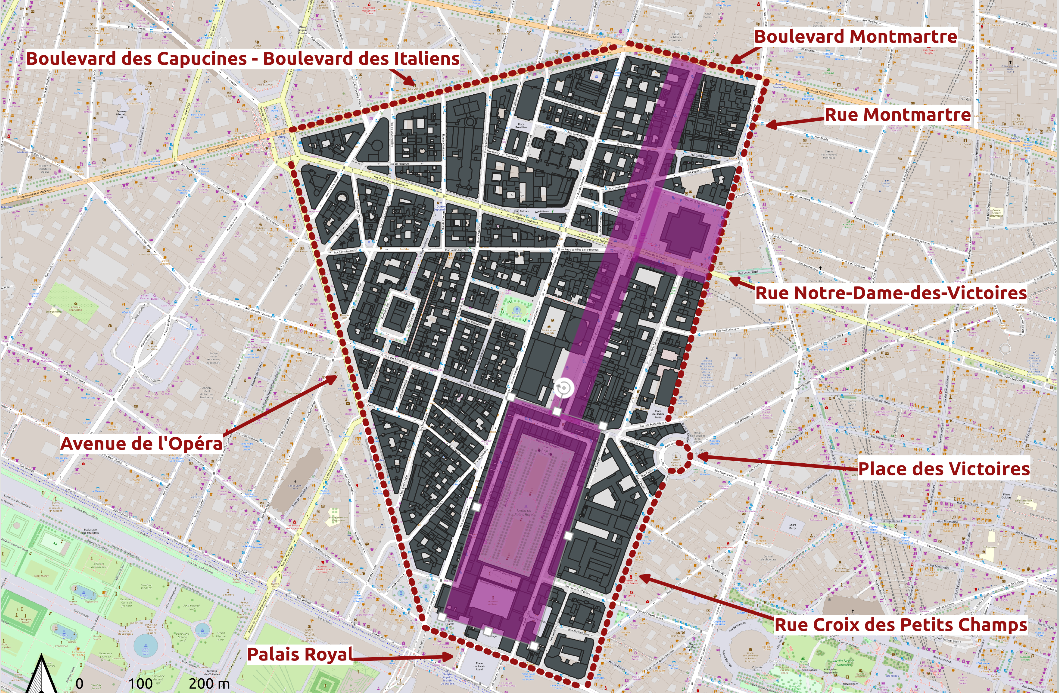
\includegraphics[width=\textwidth]{includes/topographie.png}
		\caption{La topographie du quartier Richelieu}
	\end{figure}
\end{frame}

\subsection[Une approche \textit{spatial turn}]{Une approche \textit{spatial turn}}
\begin{frame}{Aborder un quartier par le lieu}{Une approche \textit{spatial turn}}
	\begin{figure}
		\centering
		\begin{subfigure}{0.7\textwidth}
			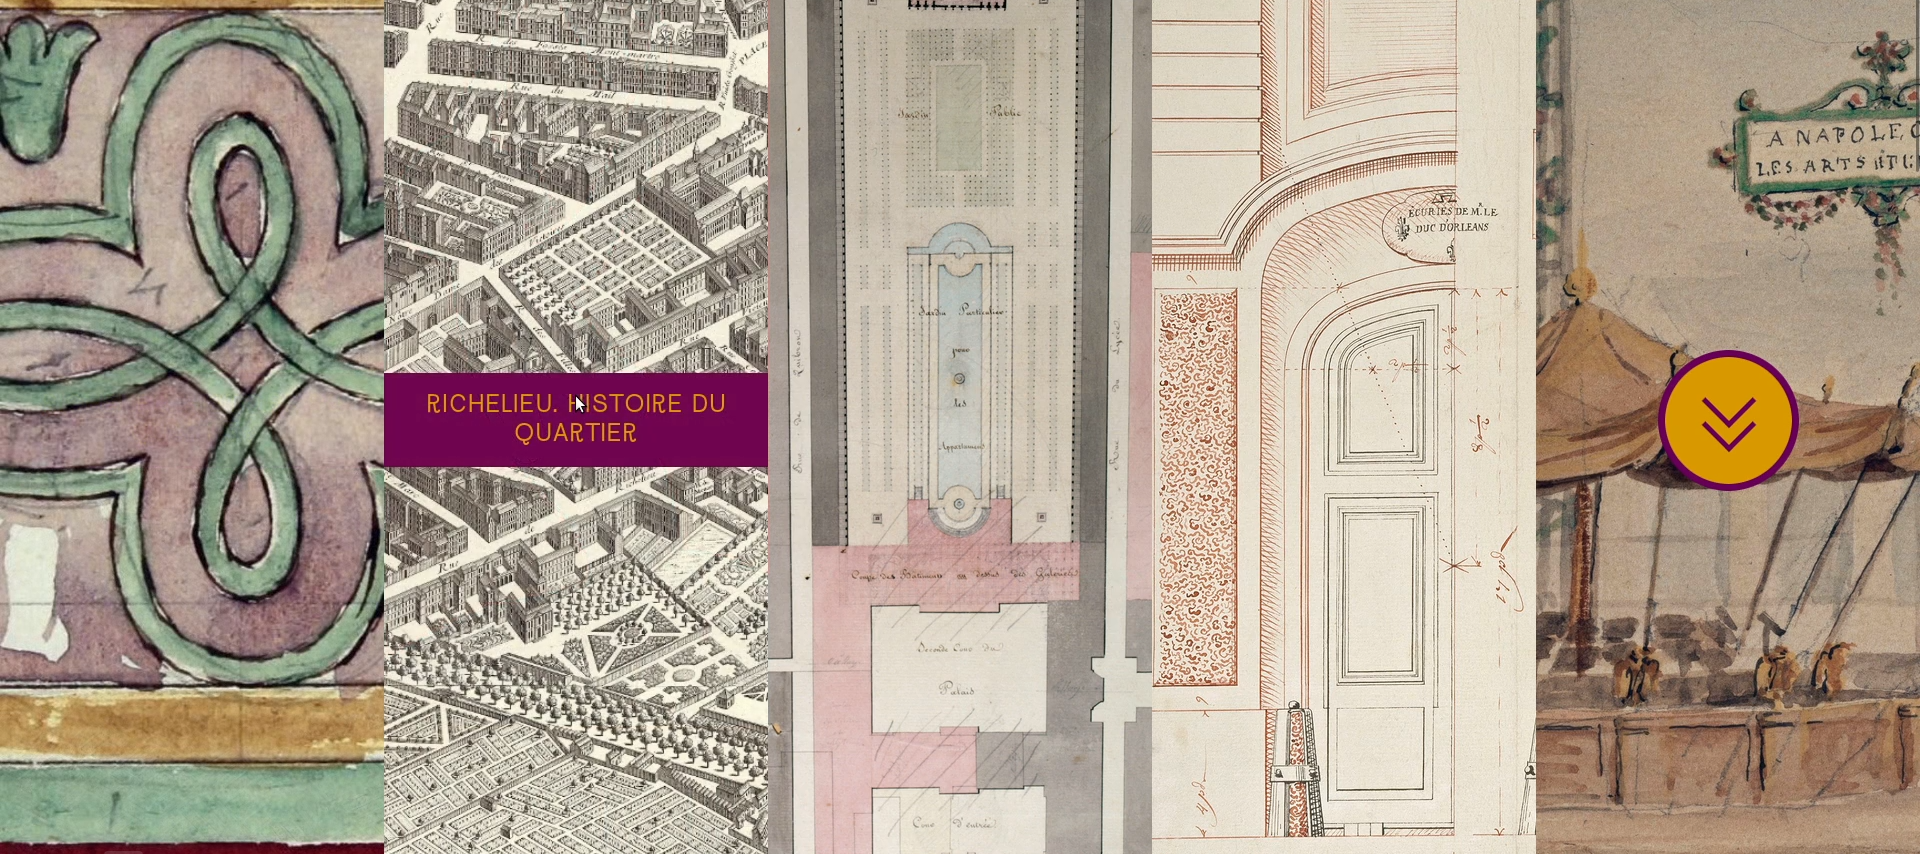
\includegraphics[width=\textwidth]{includes/app_1.png}
		\end{subfigure}
		\begin{subfigure}{0.7\textwidth}
			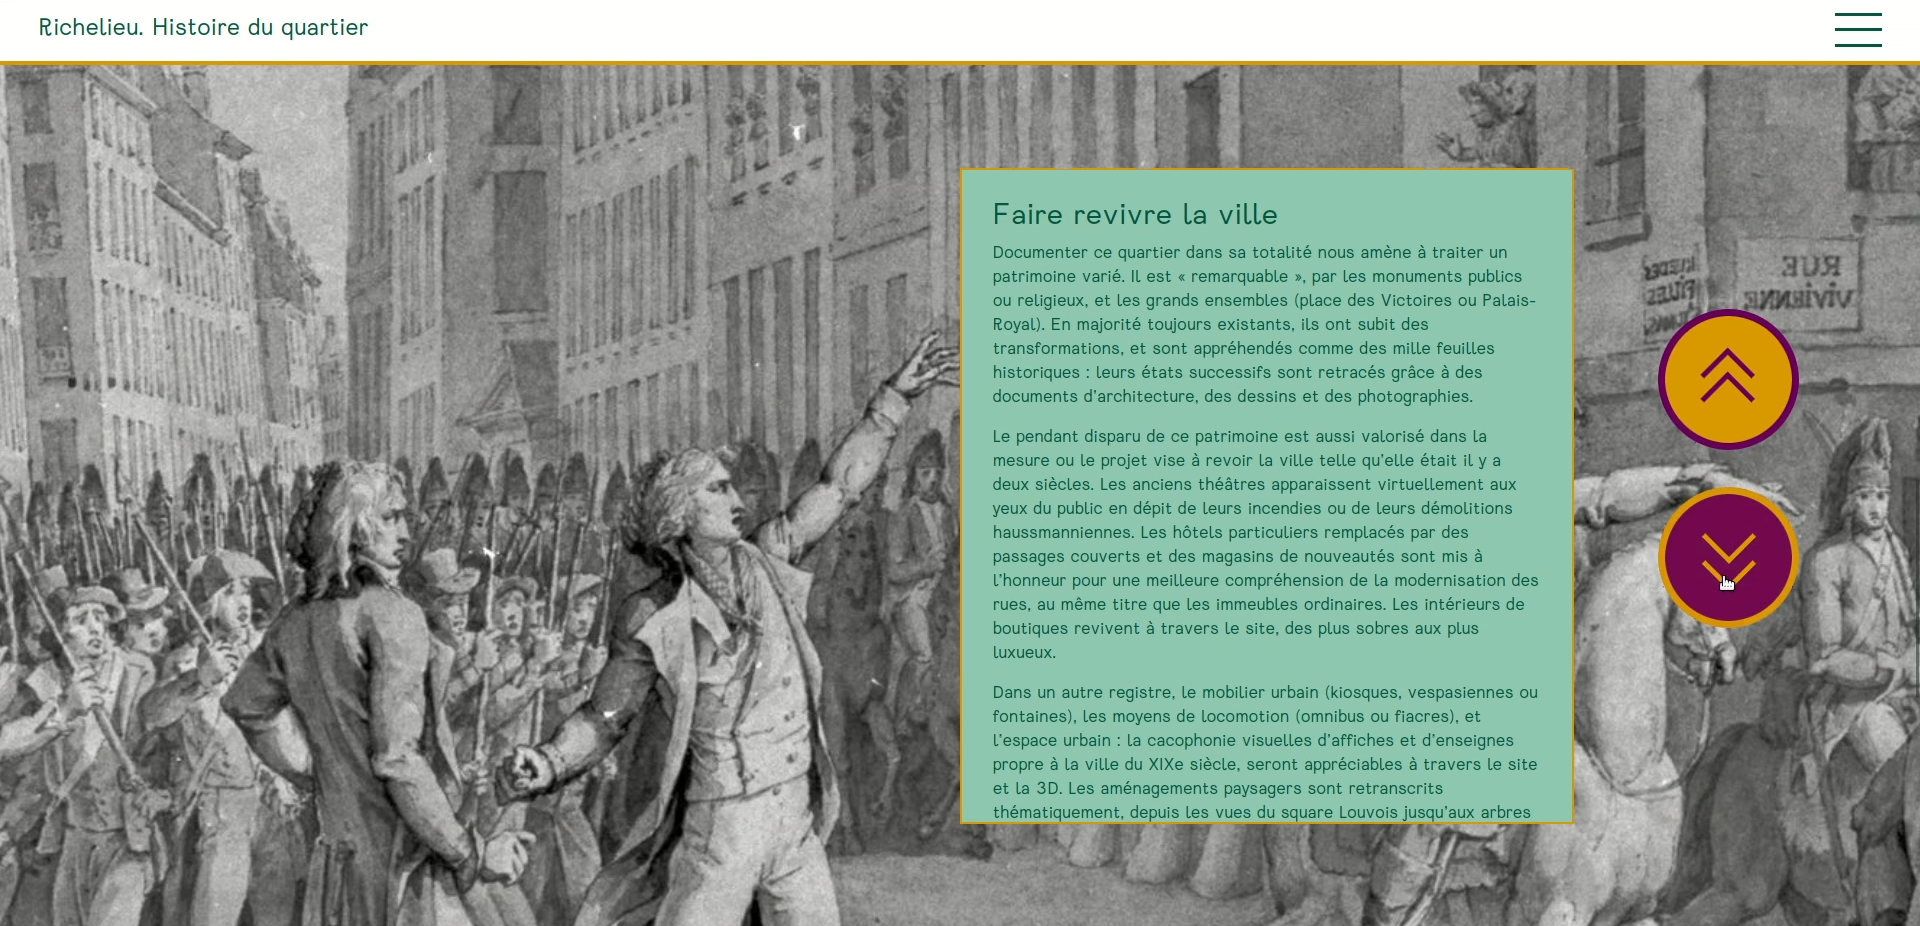
\includegraphics[width=\textwidth]{includes/app_2.png}
		\end{subfigure}
		\caption{Deux captures d'écran de l'application Web du projet \enquote{Richelieu}}
	\end{figure}
\end{frame}

% 2e slide appli

\subsection{Les dimensions du lieu}
\begin{frame}{Aborder un quartier par le lieu}{Les réseaux du quartier}
	\begin{columns}[c]
		\begin{column}{0.5\textwidth}
			\begin{tabular}{p{\textwidth}}
				\begin{figure}
				\centering
					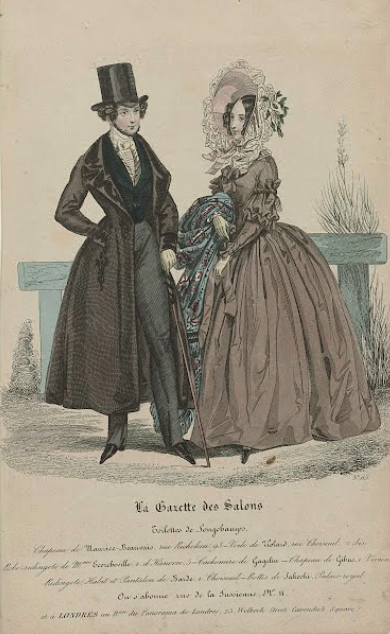
\includegraphics[width=0.7\textwidth]{includes/costume.png}
				\end{figure}
				\\ 
				\emulatecaption{La Gazette des Salons, 1836, n°115, Toilettes de Longchamp, Rijksmuseum, Amsterdam}
			\end{tabular}
		\end{column}
		\begin{column}{0.5\textwidth}
			\begin{itemize}
				\item Chapeau de Maurice-Beauvais, \textbf{93 rue Richelieu}
				\item Redingote habit et pantalon de Barbe, \textbf{Rue Choiseul}
				\item Bottes de Sakoski, \textbf{Palais-Royal}
				\item Chapeau de Gibus, \textbf{Rue Vivienne}
				\item Voile de Violard, \textbf{2 bis rue Choiseul}
				\item Robe-redingote de Mme Ecorcheville, \textbf{5 rue d’Hanovre}
			\end{itemize}		
		\end{column}
	\end{columns}
\end{frame}

\begin{frame}{Aborder un quartier par le lieu}{Les réseaux du quartier}
	\begin{figure}
		\centering
		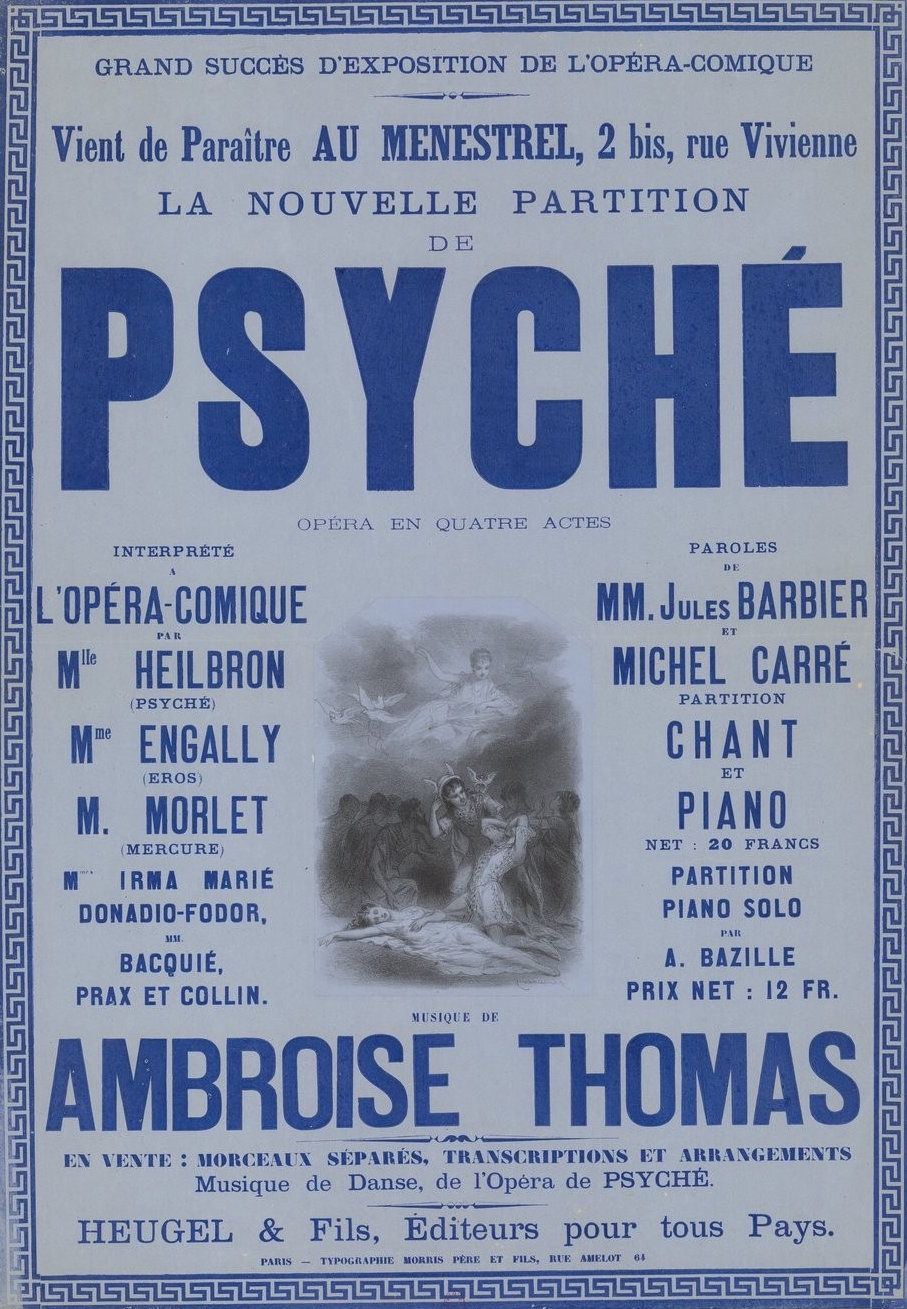
\includegraphics[height=0.65\textheight]{includes/psyche.png}
		\caption{\textit{Psyché. Opéra en quatre actes, interprété à l'Opéra–Comique...}, affiche, lithographie de Antonin-Marie Chatinière, 1878, Département bibliothèque-musée de l’Opéra, BnF. Publicité pour des imprimés en vente au \textbf{Au Ménestrel, 2 bis, rue Vivienne}}
	\end{figure}
\end{frame}

\begin{frame}{Aborder un quartier par le lieu}{Les réseaux du quartier}
	\begin{figure}
		\centering
		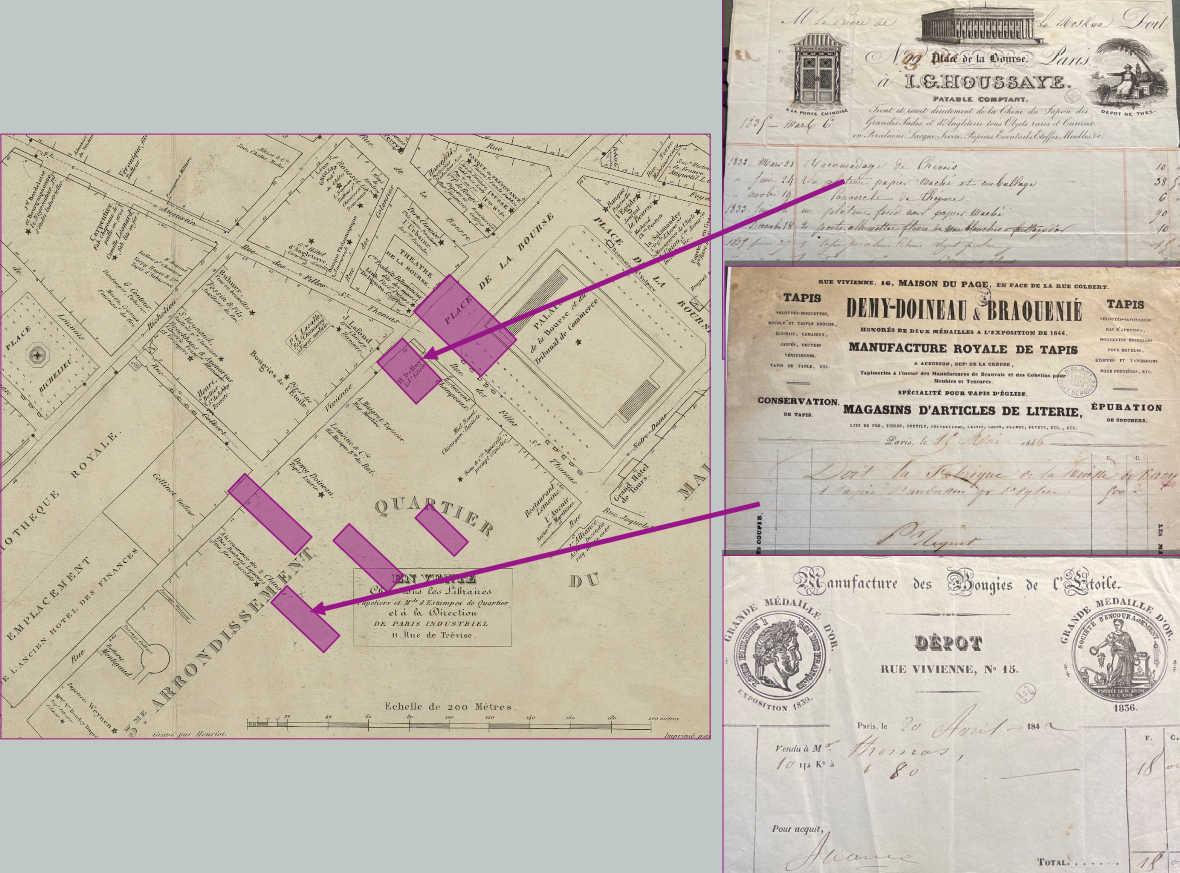
\includegraphics[width=0.9\textwidth]{includes/spatial0.png}
		\caption{Spatialisation de sources archivisitiques}
	\end{figure}
\end{frame}

\begin{frame}{Aborder un quartier par le lieu}{Histoire des mentalités}
	\begin{columns}[c]
		\begin{column}{0.5\textwidth}
			\begin{tabular}{p{\textwidth}}
				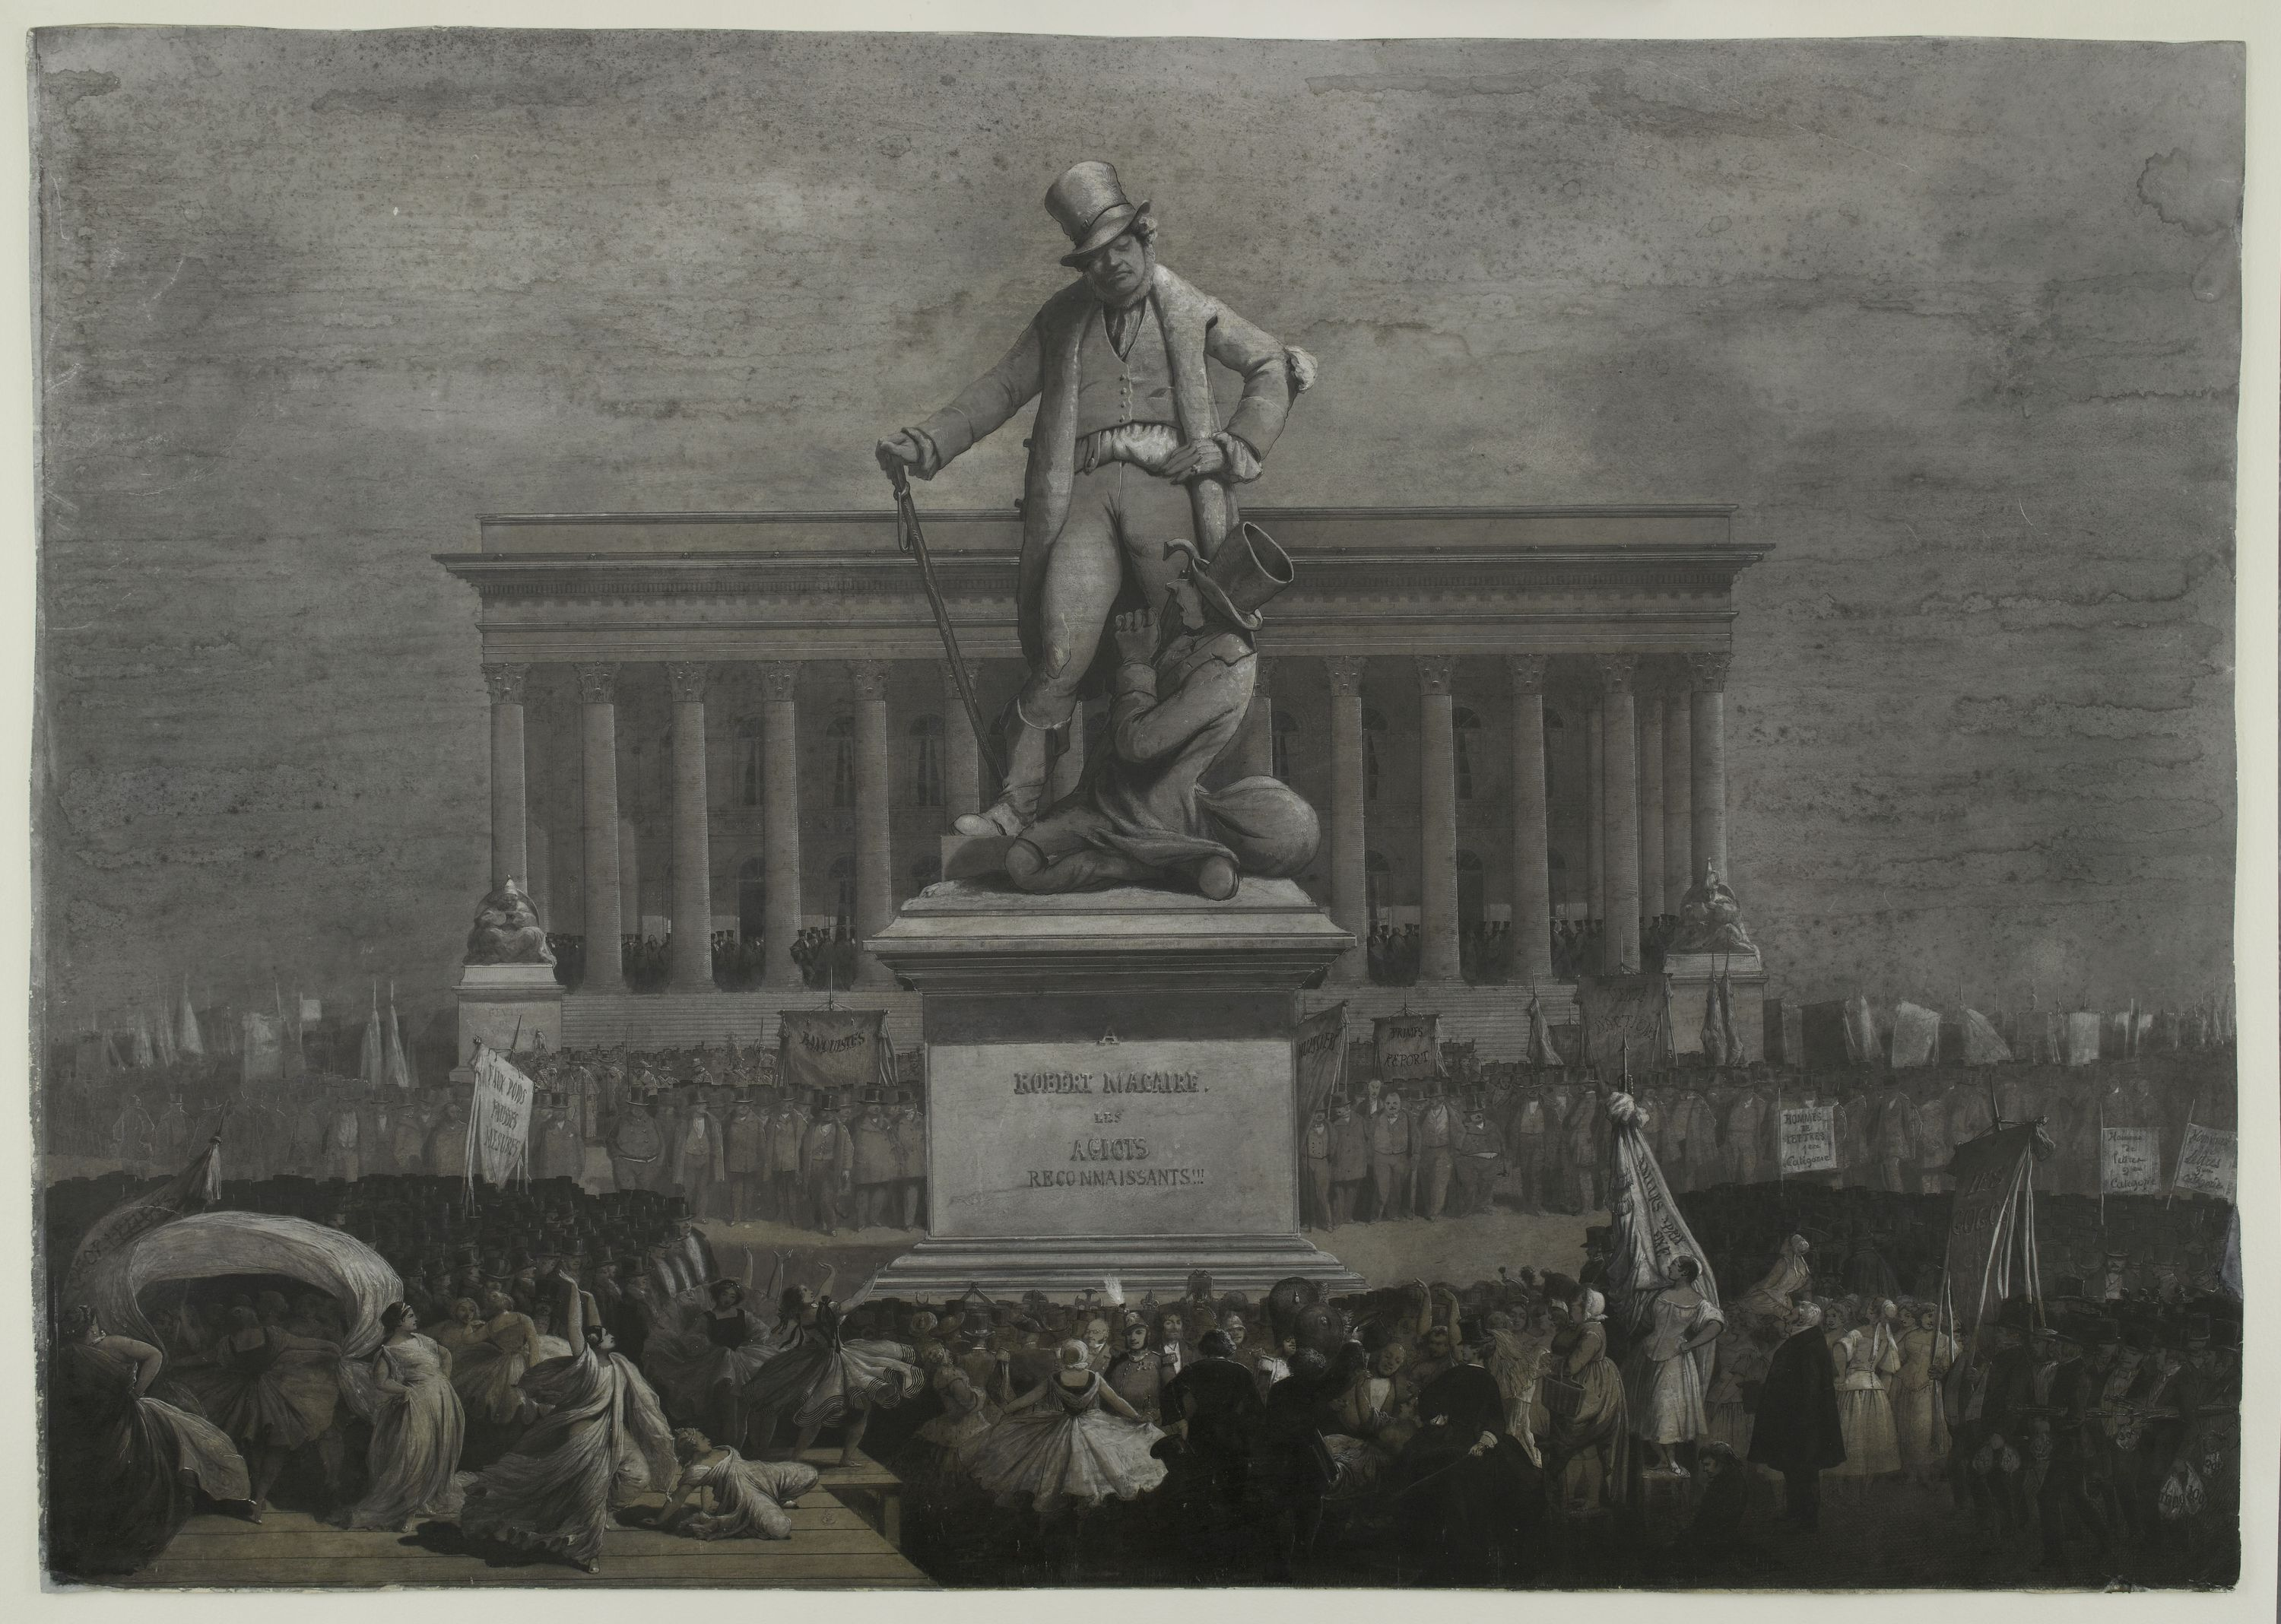
\includegraphics[height=0.27\textheight]{includes/macaire.jpg}
				\\
				\emulatecaption{Lorentz, Alcide Joseph, \textit{Monument à Robert Macaire},1856, musée Carnavalet}
				\\
				\includegraphics[height=0.27\textheight]{includes/promenade.png}
				\\
				\emulatecaption{Jean-Baptiste Arnout, \textit{Promenade pittoresque dans Paris, n° 21}, musée Carnavalet}
			\end{tabular}
		\end{column}
		\begin{column}{0.5\textwidth}
			\begin{tabular}{p{\textwidth}}
				\begin{center}
					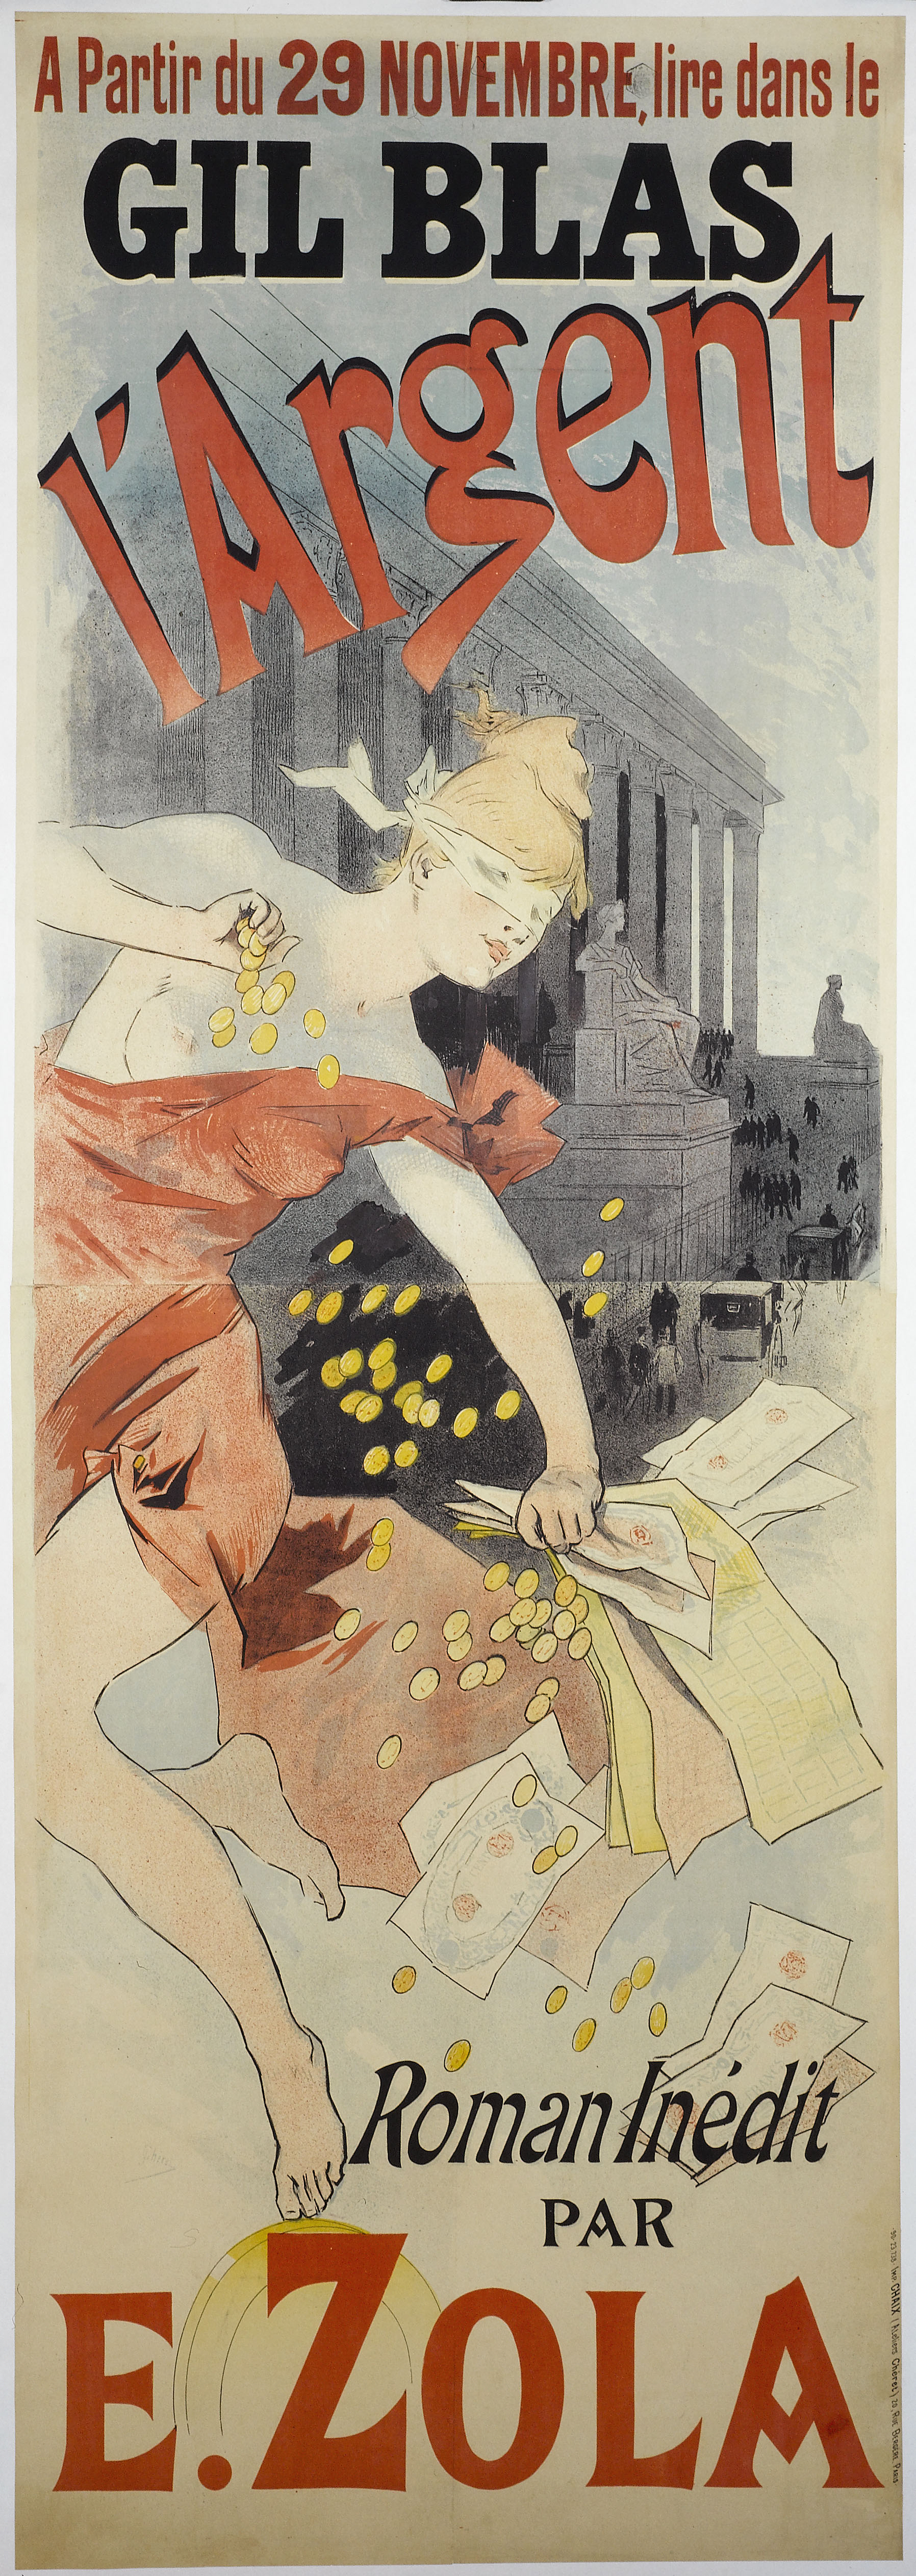
\includegraphics[height=0.63\textheight]{includes/argent.jpg}
				\end{center}
				\\
				\emulatecaption{Alcide Joseph Lorentz, \textit{Monument à Robert Macaire},1856, musée Carnavalet}
			\end{tabular}
		\end{column}
	\end{columns}
\end{frame}	

\begin{frame}{Aborder un quartier par le lieu}{Un cas d'étude: le magasin de nouveautés}
	\begin{columns}[c]
		\begin{column}{0.5\textwidth}
			\begin{tabular}{p{\textwidth}}
				\begin{center}
					\includegraphics[width=0.9\textwidth]{includes/vdf1.png}
				\end{center}
				\\
				\emulatecaption{\textit{\enquote{Aux villes de France}, n° 51 rue Vivienne, n° 104 rue Richelieu, \enquote{magasin de nouveautés le plus vaste de l’univers}}, Bibliothèque historique de la ville de Paris}
			\end{tabular}
		\end{column}
		\begin{column}{0.5\textwidth}
			\begin{tabular}{p{\textwidth}}
				\includegraphics[height=0.35\textheight]{includes/vdf2.png}
				\\
				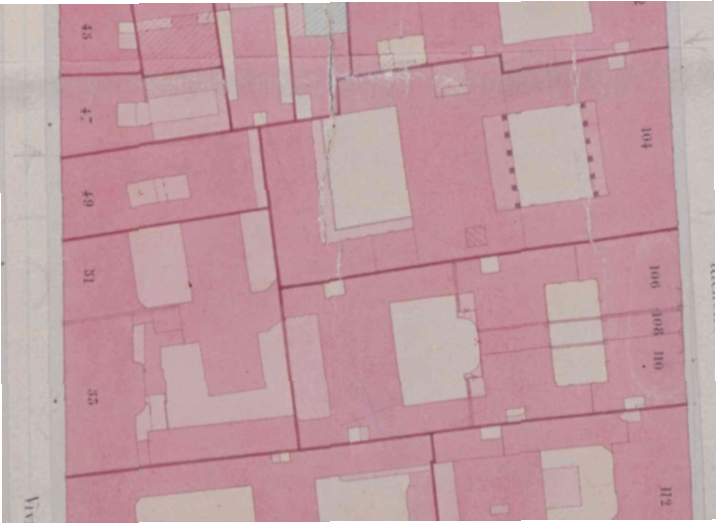
\includegraphics[height=0.35\textheight]{includes/map.png}
				\\
				\emulatecaption{\textit{Plan parcellaire municipal de Paris (fin XIX\textsuperscript{e})}, Quartier Vivienne, Archives de la Ville de Paris}
			\end{tabular}
		\end{column}
	\end{columns}
\end{frame}

\begin{frame}{Aborder un quartier par le lieu}{Spatialiser la ville rêvée}
	\begin{figure}
		\centering
		\begin{subfigure}{0.48\textwidth}
			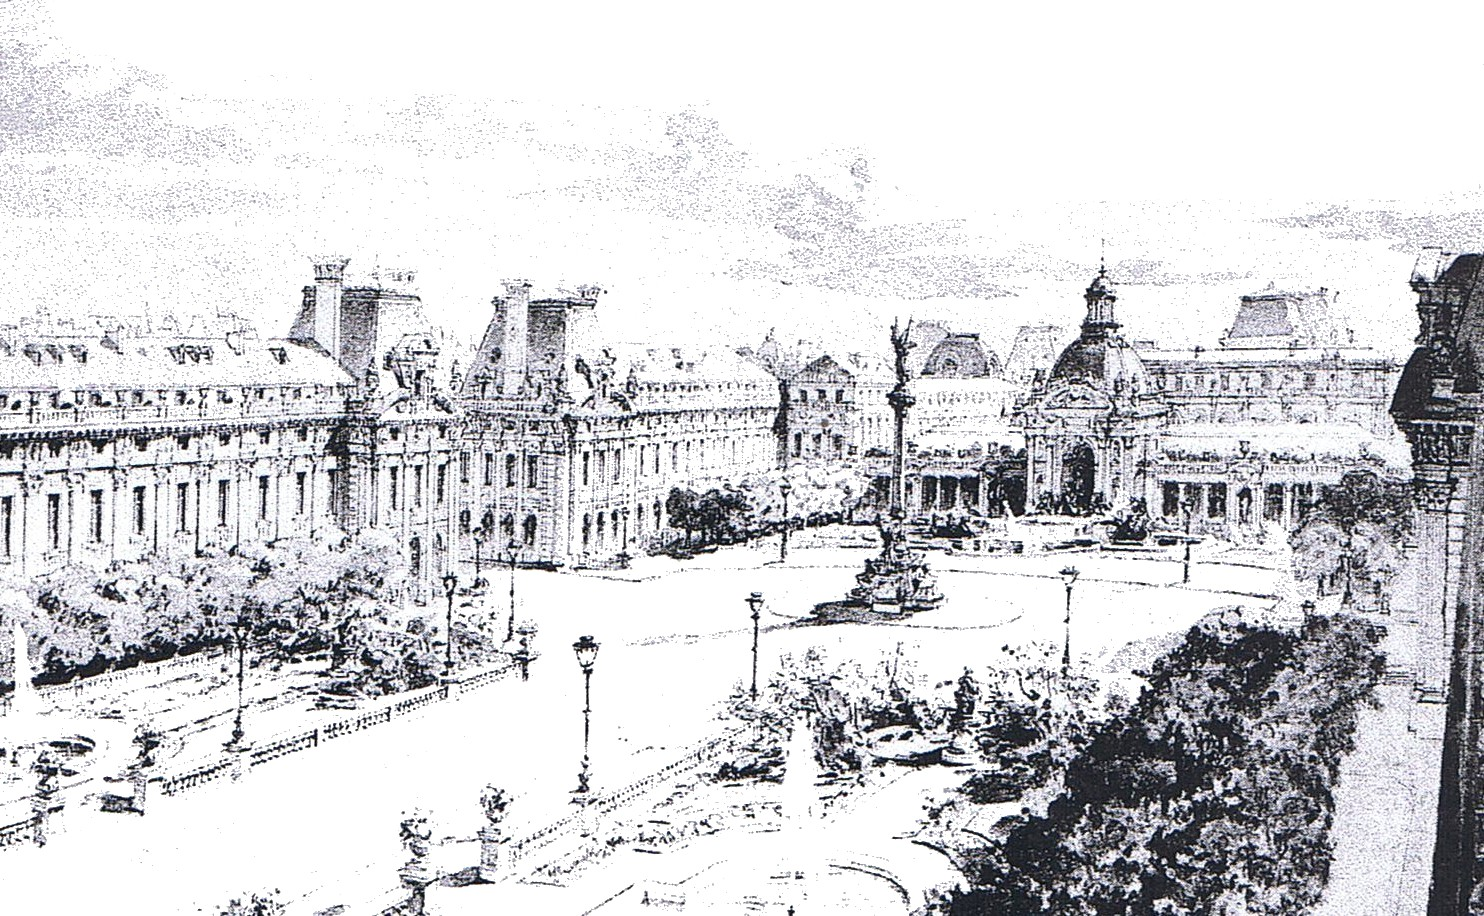
\includegraphics[width=\textwidth]{includes/pr.jpg}
			\caption{Henri Deverin, Projet de transformation du Palais-Royal, \textit{Revue l’architecture}, 1905}
		\end{subfigure}
		\hfill
		\begin{subfigure}{0.5\textwidth}
			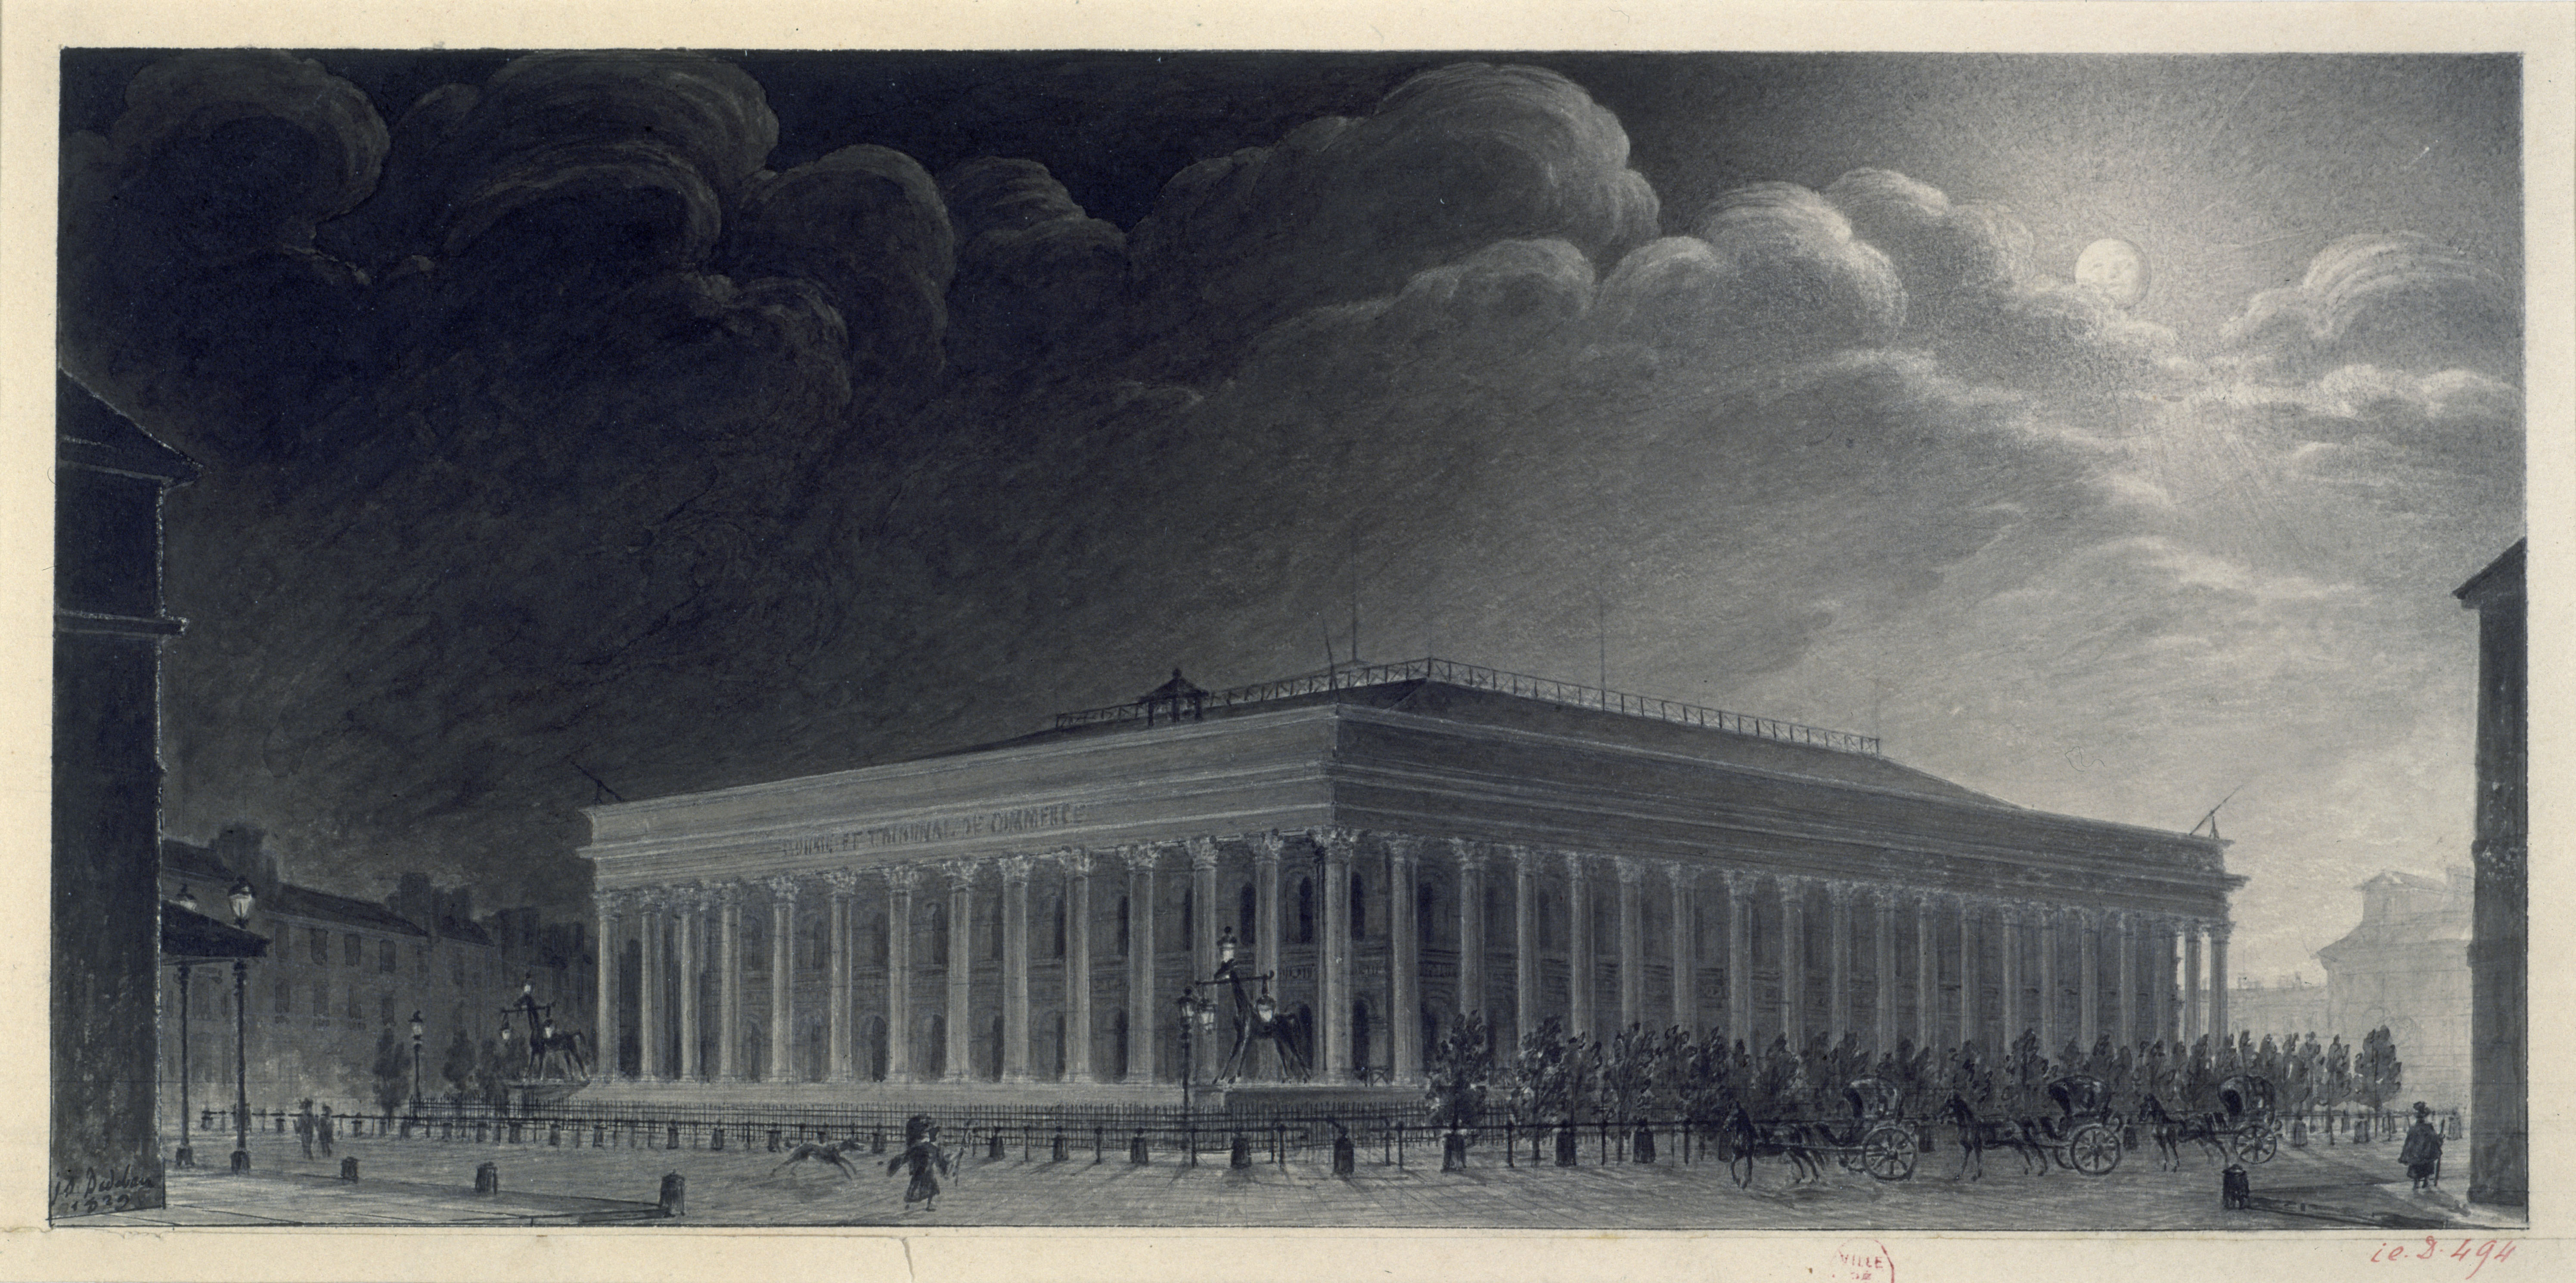
\includegraphics[width=\textwidth]{includes/pb.jpg}
			\caption{Jean-Baptiste Dedeban, \textit{Projet d’éclairage de la Bourse}, musée Carnavalet, 1829}
		\end{subfigure}
		%\hfill
		\begin{subfigure}{\textwidth}
			\centering
			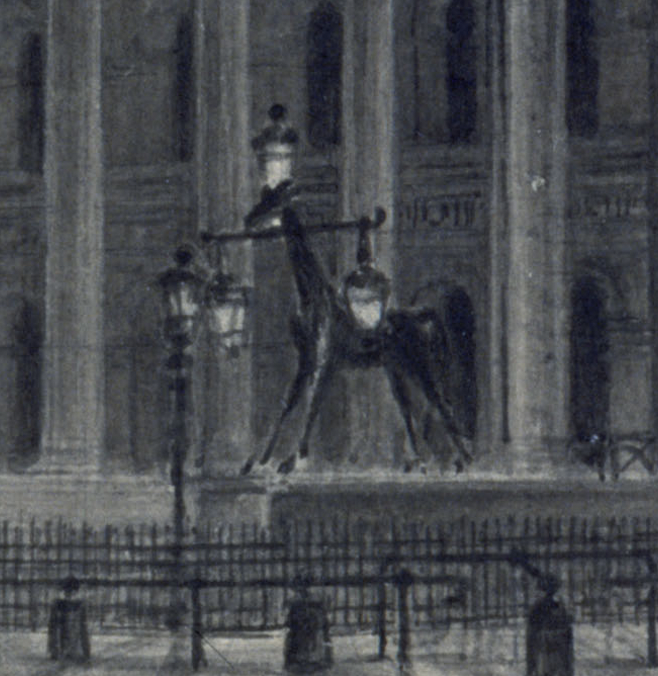
\includegraphics[width=0.25\textwidth]{includes/pb_detail.png}
			\caption{Jean-Baptiste Dedeban, \textit{Projet d’éclairage de la Bourse} (détail), musée Carnavalet, 1829}
		\end{subfigure}
	\end{figure}
\end{frame}

\begin{frame}{Aborder un quartier par le lieu}{Resituer les représentations d'un quartier dans l'espace}
	\begin{figure}
		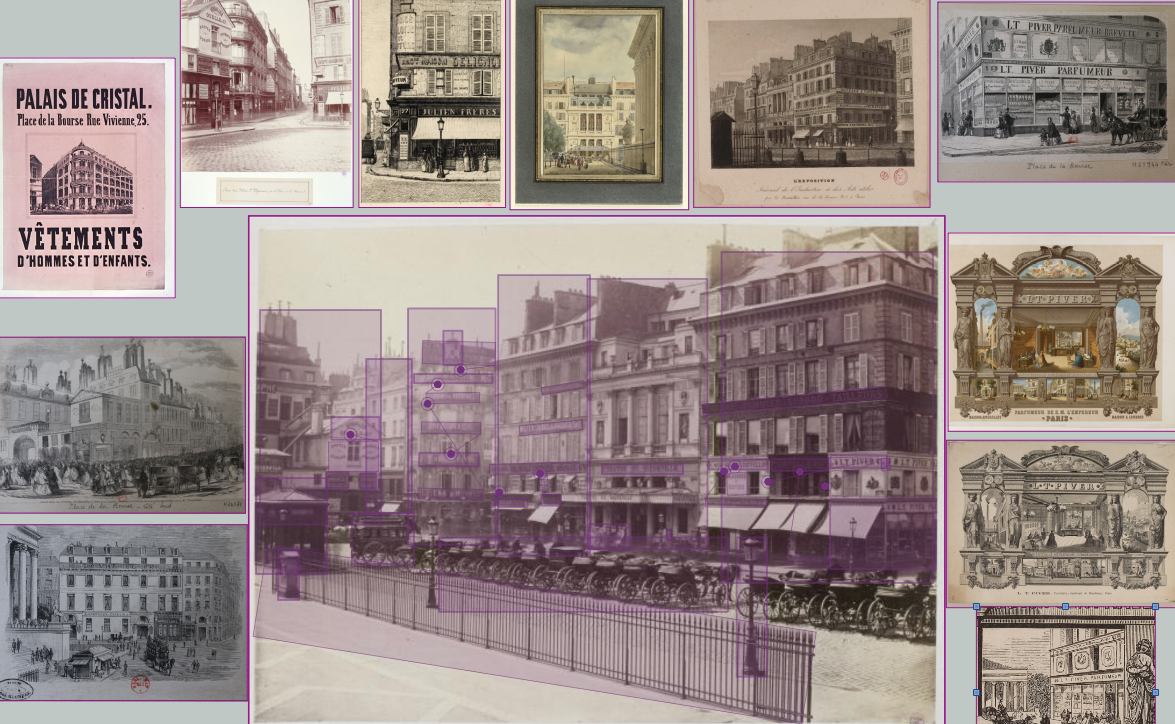
\includegraphics[width=\textwidth]{includes/final_cha.png}
	\end{figure}
\end{frame}

\section{Modéliser un lieu, structurer une pluralité}
\subsection[Une réponse technique]{Une réponse technique à des questionnements théoriques}
\begin{frame}{Modéliser un lieu, structurer une pluralité}{Une réponse technique à des questionnements théoriques}
	Les réflexions sur le lieu \textbf{structurent toute la chaîne de traitement} du projet Richelieu et sont centrales sur \textbf{trois plans}:
	\begin{itemize}
		\item La modélisation des données
		\item La modélisation 3D de la Place de la Bourse
		\item Le développement de l'application Web du projet
	\end{itemize}
	\begin{figure}
		\includegraphics[width=\textwidth]{includes/pipeline-richelieu.png}
		\caption{Chaîne de traitement du projet}
	\end{figure}
\end{frame}


\subsection[Des unités minimales]{Des unités minimales en interrelation: une approche modulaire du lieu}
\begin{frame}{Modéliser un lieu, structurer une pluralité}{Des unités minimales en interrelation: une approche modulaire du lieu}
	Un modèle relationnel (\texttt{SQL}) permet une approche \textbf{modulaire} du lieu:
	\begin{itemize}
		\item Pas du \enquote{sujet} central (contrairement au \texttt{XML})
		\item Le domaine modélisé est divisé en une collection d'objets en interrelation
		\item Plusieurs vues d'un même objet sont possibles
	\end{itemize}
	Le modèle relationnel permet donc de modéliser la complexité du lieu en l'abordant comme un ensemble d'\textbf{unités minimales en interrelation}.
\end{frame}

\begin{frame}{Modéliser un lieu, structurer une pluralité}{Des unités minimales en interrelation: une approche modulaire du lieu}
	\begin{figure}[width=\textwidth,height=\textheight]
		\centering
		\tikz[node distance=1cm, scale=0.7, transform shape]{
			\node[act] (lieu) at (0,0) 
			{
				\tikztemplate{Lieu}{
					\begin{itemize}
						\item Emprise au sol
						\item Durée d'existence (tranche de dates)
					\end{itemize}
				}
			};
		}
		\caption{Model conceptuel d'un lieu (simplifié)}
	\end{figure}
\end{frame}

\begin{frame}{Modéliser un lieu, structurer une pluralité}{Des unités minimales en interrelation: une approche modulaire du lieu}
	\begin{figure}[width=\textwidth,height=\textheight]
		\centering
		\tikz[node distance=1cm, scale=0.7, transform shape]{
			\node[act] (lieu) at (0,0) 
			{
				\tikztemplate{Lieu}{
					\begin{itemize}
						\item Emprise au sol
						\item Durée d'existence (tranche de dates)
					\end{itemize}
				}
			};
			\node[act] (addresse) at (5,0) 
			{
				\tikztemplate{Adresse}{
					Désignation administrative du lieu
					\begin{itemize}
						\item N° de rue
						\item Nom de rue
					\end{itemize}
				}
			};
			\draw[arrow] (lieu) -- (addresse);
		}
		\caption{Model conceptuel d'un lieu (simplifié)}
	\end{figure}
\end{frame}

\begin{frame}{Modéliser un lieu, structurer une pluralité}{Des unités minimales en interrelation: une approche modulaire du lieu}
	\begin{figure}[width=\textwidth,height=\textheight]
		\centering
		\tikz[node distance=1cm, scale=0.7, transform shape]{
			\node[act] (lieu) at (0,0) 
			{
				\tikztemplate{Lieu}{
					\begin{itemize}
						\item Emprise au sol
						\item Durée d'existence (tranche de dates)
					\end{itemize}
				}
			};
			\node[act] (addresse) at (5,0) 
			{
				\tikztemplate{Adresse}{
					Désignation administrative du lieu
					\begin{itemize}
						\item N° de rue
						\item Nom de rue
					\end{itemize}
				}
			};
			\node[act] (carte) at (0,-3) 
			{
				\tikztemplate{Cartographie}{
					Représentation cartographique du lieu dans un document d'archives
					\begin{itemize}
						\item Cartel muséographique
						\item Lien le fichier image spatialisé dans un SIG
					\end{itemize}
				}
			};
			\draw[arrow] (lieu) -- (addresse);
			\draw[arrow] (lieu) -- (carte);
		}
		\caption{Model conceptuel d'un lieu (simplifié)}
	\end{figure}
\end{frame}

\begin{frame}{Modéliser un lieu, structurer une pluralité}{Des unités minimales en interrelation: une approche modulaire du lieu}
	\begin{figure}[width=\textwidth,height=\textheight]
		\centering
		\tikz[node distance=1cm, scale=0.7, transform shape]{
			\node[act] (lieu) at (0,0) 
			{
				\tikztemplate{Lieu}{
					\begin{itemize}
						\item Emprise au sol
						\item Durée d'existence (tranche de dates)
					\end{itemize}
				}
			};
			\node[act] (addresse) at (5,0) 
			{
				\tikztemplate{Adresse}{
					Désignation administrative du lieu
					\begin{itemize}
						\item N° de rue
						\item Nom de rue
					\end{itemize}
				}
			};
			\node[act] (carte) at (0,-3) 
			{
				\tikztemplate{Cartographie}{
					Représentation cartographique du lieu dans un document d'archives
					\begin{itemize}
						\item Cartel muséographique
						\item Lien le fichier image spatialisé dans un SIG
					\end{itemize}
				}
			};
			\node[act] (icono) at (-5,0) 
			{
				\tikztemplate{Iconographie}{
					Ressource iconographique représentant du lieu
					\begin{itemize}
						\item Cartel muséographique
						\item Lien vers des manifestes IIIF pour accéder aux images
					\end{itemize}
				}
			};
			\draw[arrow] (lieu) -- (addresse);
			\draw[arrow] (lieu) -- (carte);
			\draw[arrow] (lieu) -- (icono);
		}
		\caption{Model conceptuel d'un lieu (simplifié)}
	\end{figure}
\end{frame}

\begin{frame}{Modéliser un lieu, structurer une pluralité}{Des unités minimales en interrelation: une approche modulaire du lieu}
	\begin{figure}[width=\textwidth,height=\textheight]
		\centering
		\tikz[node distance=1cm, scale=0.7, transform shape]{
			\node[act] (lieu) at (0,0) 
			{
				\tikztemplate{Lieu}{
					\begin{itemize}
						\item Emprise au sol
						\item Durée d'existence (tranche de dates)
					\end{itemize}
				}
			};
			\node[act] (addresse) at (5,0) 
			{
				\tikztemplate{Adresse}{
					Désignation administrative du lieu
					\begin{itemize}
						\item N° de rue
						\item Nom de rue
					\end{itemize}
				}
			};
			\node[act] (carte) at (0,-3) 
			{
				\tikztemplate{Cartographie}{
					Représentation cartographique du lieu dans un document d'archives
					\begin{itemize}
						\item Cartel muséographique
						\item Lien le fichier image spatialisé dans un SIG
					\end{itemize}
				}
			};
			\node[act] (icono) at (-5,0) 
			{
				\tikztemplate{Iconographie}{
					Ressource iconographique représentant du lieu
					\begin{itemize}
						\item Cartel muséographique
						\item Lien vers des manifestes IIIF pour accéder aux images
					\end{itemize}
				}
			};
			\node[act] (groupe) at (0,2.5) 
			{
				\tikztemplate{Groupement de lieux}{
					Groupement synchronique des évolutions d'un lieu dans le temps
				}
			};
			\draw[arrow] (lieu) -- (addresse);
			\draw[arrow] (lieu) -- (carte);
			\draw[arrow] (lieu) -- (groupe);
			\draw[arrow] (lieu) -- (icono);
		}
		\caption{Model conceptuel d'un lieu (simplifié)}
	\end{figure}
\end{frame}

\begin{frame}{Modéliser un lieu, structurer une pluralité}{Des unités minimales en interrelation: une approche modulaire du lieu}
	\begin{figure}[width=\textwidth,height=\textheight]
		\centering
		\includegraphics[width=0.9\textwidth]{includes/data-model.png}
		\caption{Modèle relationnel complet de la base de données Richelieu}
	\end{figure}
\end{frame}

\subsection[Modélisation partielle]{Modélisation partielle et angles morts}
\begin{frame}{Modéliser un lieu, structurer une pluralité}{Modélisation partielle et angles morts}
	Notre approche du lieu est pragmatique et laisse des angles morts:
	\begin{itemize}
		\item Contraintes techniques
		\item Espace bidimensionnel
	\end{itemize}
\end{frame}

\section{Restituer un lieu: des sources à la modélisation 3D}
\subsection{Quelles sources pour la 3D?}
\begin{frame}{Restituer un lieu: la modélisation 3D}{Quelles sources pour la 3D?}
	\begin{columns}[c]
		\begin{column}{0.5\textwidth}
			\small
				\textit{\enquote{J'aimerais qu’il existe des lieux stables, immobiles, intangibles, intouchés et presque intouchables, immuables, enracinés; des lieux qui seraient des références, des points de départ, des sources.}}
			
				\textit{\enquote{[...] De tels lieux n’existent pas, et c’est parce qu’ils n'existent pas que l’espace devient question, cesse d’être une évidence, cesse d'être incorporé, cesse d'être approprié. L’espace est un doute: il faut sans cesse le marquer, le désigner; il n’est jamais à moi, il ne m’est jamais donné, il faut que j’en fasse la conquête.}}	
			
				\textit{\enquote{[…] L'espace fond comme le sable coule entre les doigts. Le temps l’emporte et ne m’en laisse que des lambeaux informes...}}
			
			\normalsize
			-- Georges Perec, \textit{Espèces d’espaces}, Paris, Galilée, 1974, p. 122-123.
		\end{column}
		\begin{column}{0.5\textwidth}
			\begin{figure}
				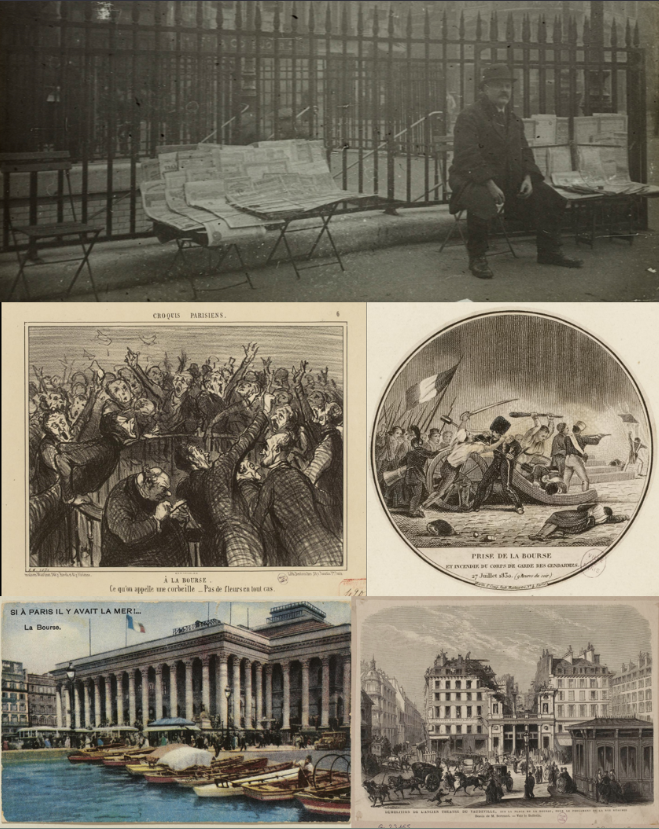
\includegraphics[width=\textwidth]{includes/c_slide0.png}
			\end{figure}
		\end{column}
	\end{columns}
\end{frame}

\begin{frame}{Restituer un lieu: des sources à la modélisation 3D}{Quelles sources pour la 3D?}
	\begin{columns}[c]
		\begin{column}{0.5\textwidth}
			Des sources de \textbf{nature, fiabilité et précision multiples}:
			\begin{itemize}
				\item Plans de censive, documents fiscaux levés ou non par des géomètres
				\item Atlas, documents levés à l’échelle de la ville, eux aussi à précision variable
				\item Plans d’expropriation ou d’alignement, utilisés par les urbanistes et les services municipaux, très précis
				\item Plans d’ensemble à l’usage du public, à destination commerciale, touristique, explicative souvent sans grand souci de précision
			\end{itemize}
			Cette hétérogénéité des sources pose de nombreuses questions quant à la façon de les exploiter et nécessite une documentation de l’incertitude
		\end{column}
		\begin{column}{0.5\textwidth}
			\begin{figure}
				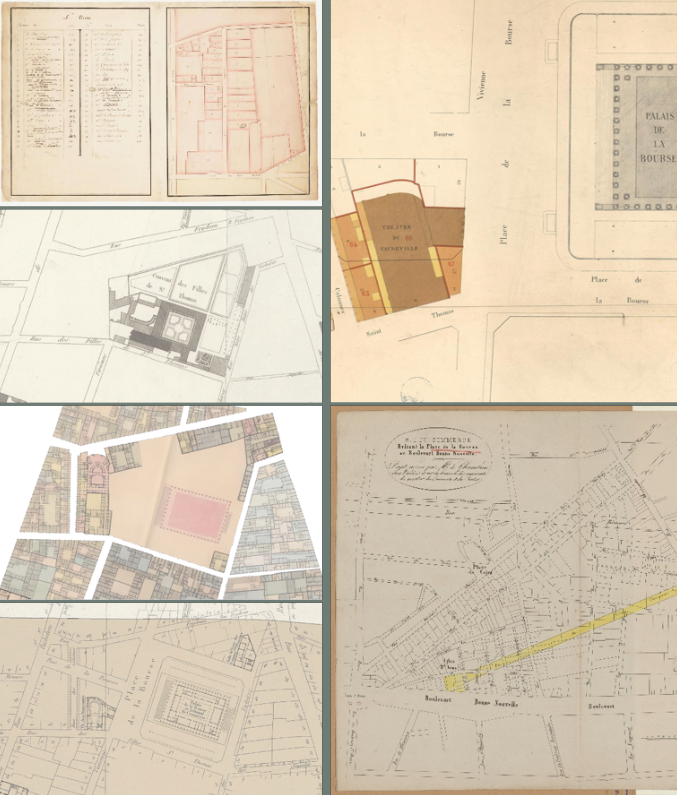
\includegraphics[width=\textwidth]{includes/c_slide1.png}
			\end{figure}
		\end{column}
	\end{columns}
\end{frame}

\subsection{Des sources à la 3D}
\begin{frame}{Restituer un lieu: des sources à la modélisation 3D}{Des sources au SIG}
	\begin{figure}
		\begin{subfigure}{0.48\textwidth}
			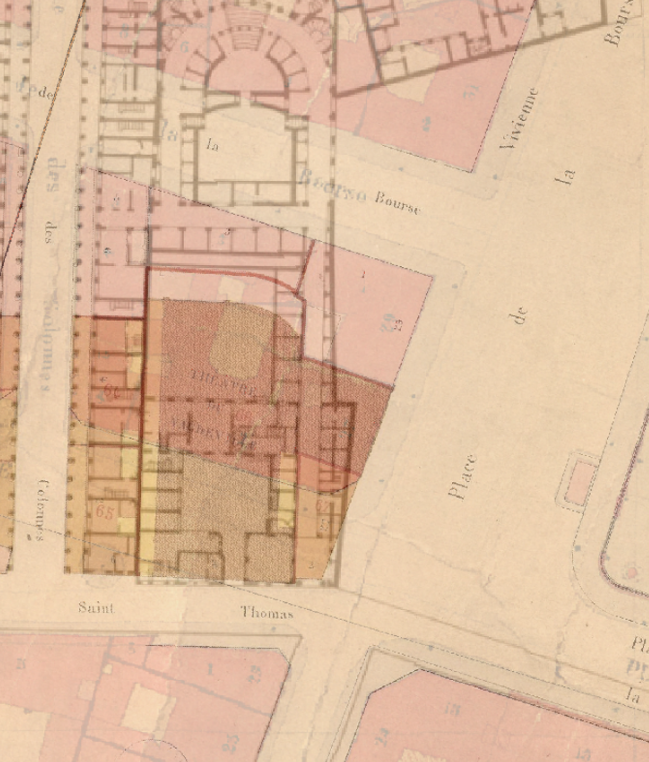
\includegraphics[width=\textwidth]{includes/c_slide2_0.png}
			\caption{Démarche de géoréférencement régressive}
		\end{subfigure}
		\begin{subfigure}{0.48\textwidth}
			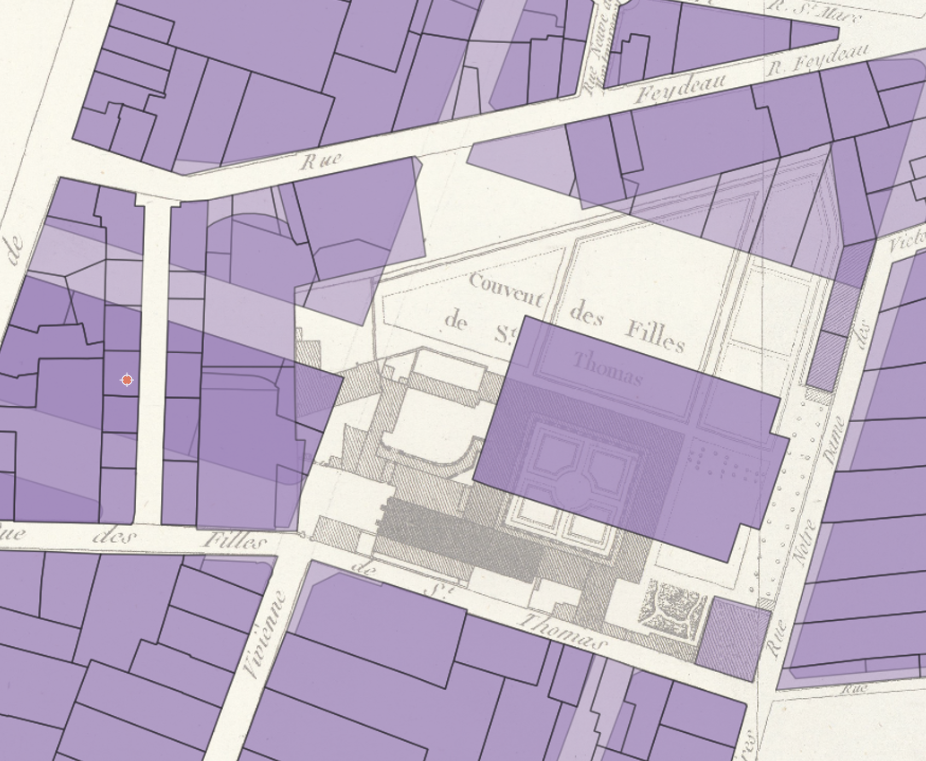
\includegraphics[width=\textwidth]{includes/c_slide2_1.png}
			\caption{Vectorisation des plans pour l’analyse spatiale}
		\end{subfigure}
	\end{figure}
\end{frame}

\begin{frame}{Restituer un lieu: des sources à la modélisation 3D}{Mutations et transmissions}
	\begin{columns}[c]
		\begin{column}{0.5\textwidth}
			On peut ensuite modéliser la stratigraphie de la ville pour rendre compte de son \enquote{épaisseur} chronologique:
			\begin{itemize}
				\item Pour étudier, caractériser comprendre la transmission des formes
				\item Pour visualiser l’aspect lacunaire des sources et les mettre en regard
				\item Pour identifier l’évolution de certaines caractéristiques du bâti (densité, surface, occupation…)
			\end{itemize}
			Cette structure en arbre reprend donc la modélisation du lieu dans la base de données
		\end{column}
		\begin{column}{0.5\textwidth}
			\begin{figure}
				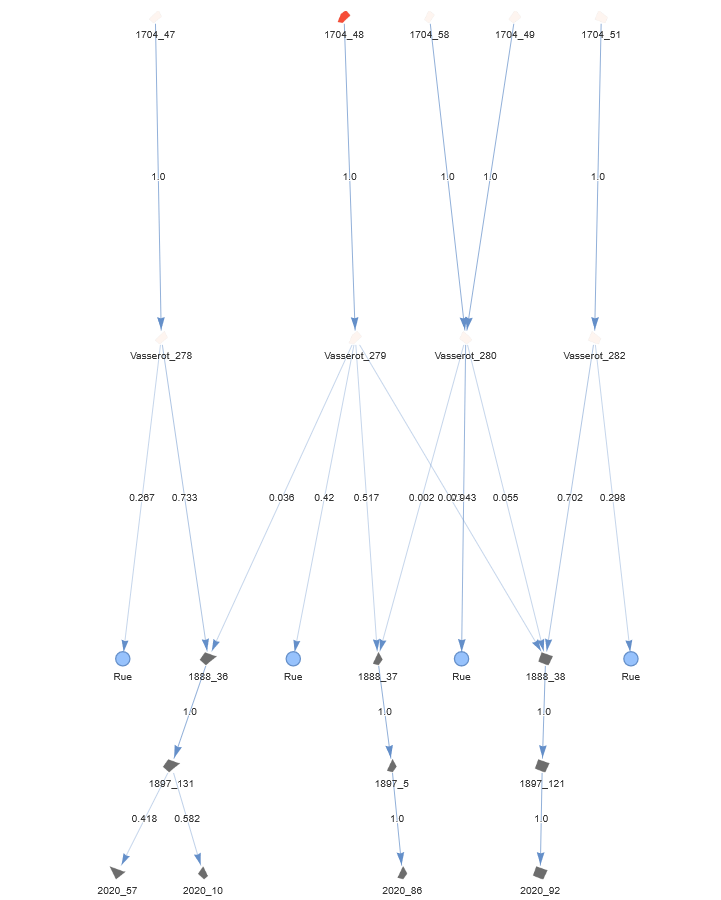
\includegraphics[width=\textwidth]{includes/c_slide3.png}
				\caption{Modéliser les mutations du parcellaire}
			\end{figure}
		\end{column}
	\end{columns}
\end{frame}

\begin{frame}{Restituer un lieu: des sources à la modélisation 3D}{Spatialisation des sources}
	\begin{figure}
		\begin{subfigure}{\textwidth}
			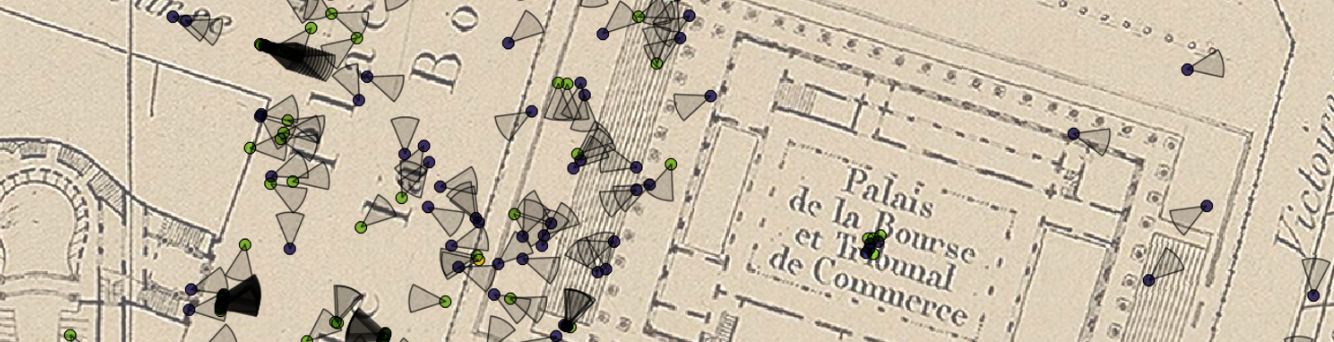
\includegraphics[width=\textwidth]{includes/c_slide4_0.png}
			\vspace{0.5cm}	
		\end{subfigure}
		\begin{subfigure}{0.4\textwidth}
			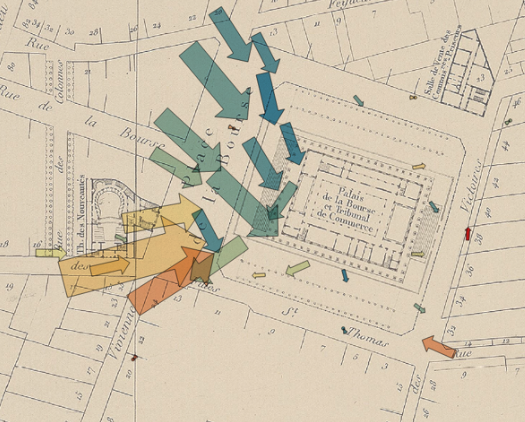
\includegraphics[width=\textwidth]{includes/c_slide4_1.png}
		\end{subfigure}
		\begin{subfigure}{0.45\textwidth}
			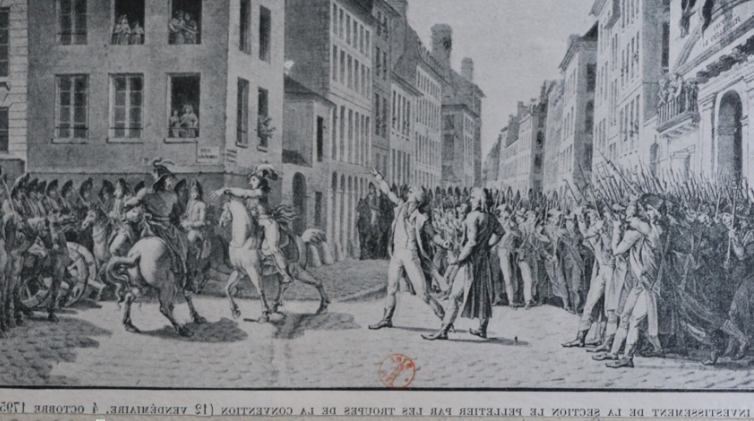
\includegraphics[width=\textwidth]{includes/c_slide4_2.png}
		\end{subfigure}
	\end{figure}
\end{frame}

\begin{frame}{Restituer un lieu: des sources à la modélisation 3D}{Les sources et l'espace}
	\begin{columns}[c]
		\begin{column}{0.4\textwidth}
			L’aspect hétérogène des sources est particulièrement visible dans leur rapport à l’espace et impose certaines \textbf{contraintes}:
			\begin{itemize}
				\item Toutes les sources ne seront pas datables et spatialisables
				\item Il faudra qualifier, de façon empirique, la représentation que la source offre de l’espace (critères de fiabilité et de lisibilité)
			\end{itemize}
			Ces contraintes rendent complexe un traitement automatique de la spatialisation des sources
		\end{column}
		\begin{column}{0.6\textwidth}
			\begin{figure}
				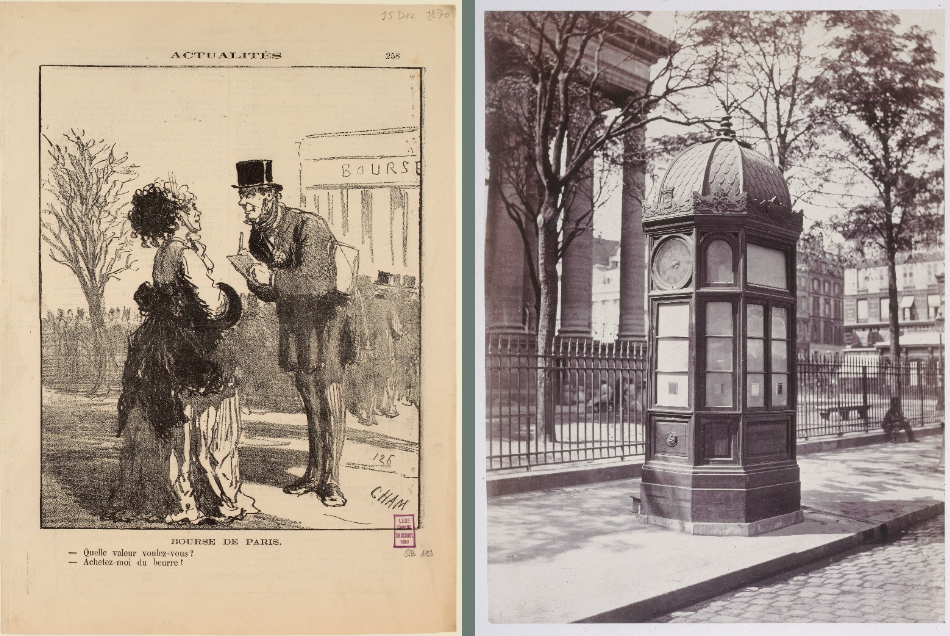
\includegraphics[width=\textwidth]{includes/c_slide5.png}
			\end{figure}	
		\end{column}
	\end{columns}
\end{frame}

\begin{frame}{Restituer un lieu: des sources à la modélisation 3D}{Quelle structure pour les sources?}
	\begin{columns}[c]
		\begin{column}{0.4\textwidth}
			La mise en relation entre les sources permet de faire une \textbf{première analyse sur leur relation au lieu}:
			\begin{itemize}
				\item 147 différents clusters dans l’iconographie, dont 57 contenant 75\% des documents
				\item On peut aussi identifier l’ordre de traitement des documents pour la modélisation en procédant de proche en proche
			\end{itemize}
		\end{column}
		\begin{column}{0.6\textwidth}
			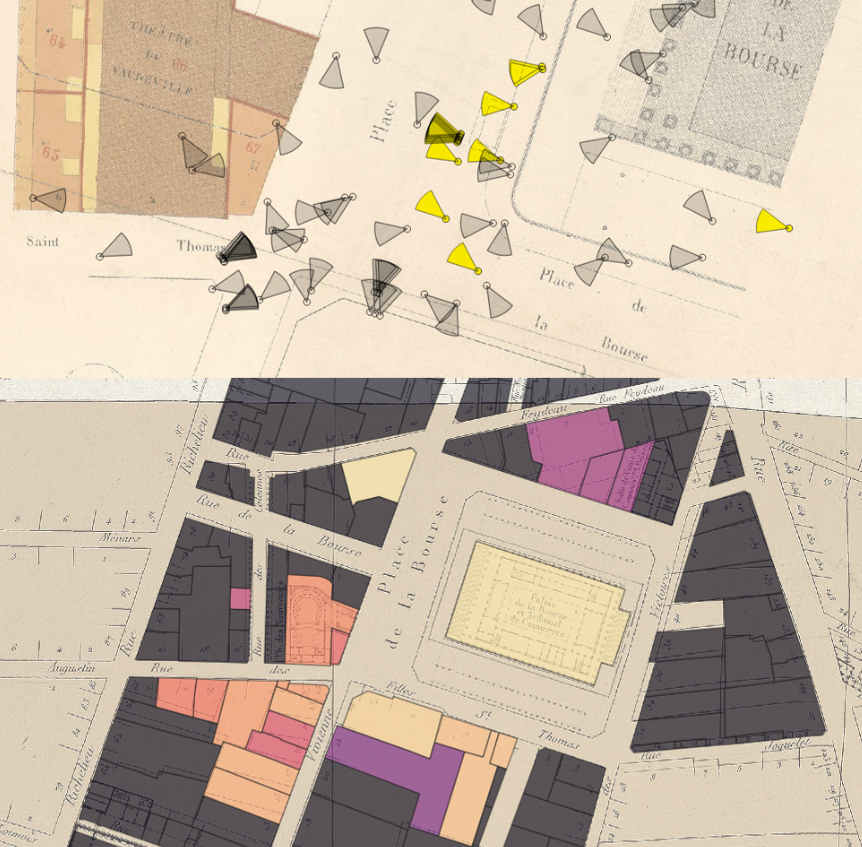
\includegraphics[width=\textwidth]{includes/c_slide6.png}
		\end{column}
	\end{columns}
\end{frame}

\begin{frame}{Restituer un lieu: des sources à la modélisation 3D}{La rue du Quatre Septembre}
	\begin{figure}
		\begin{subfigure}{0.48\textwidth}
			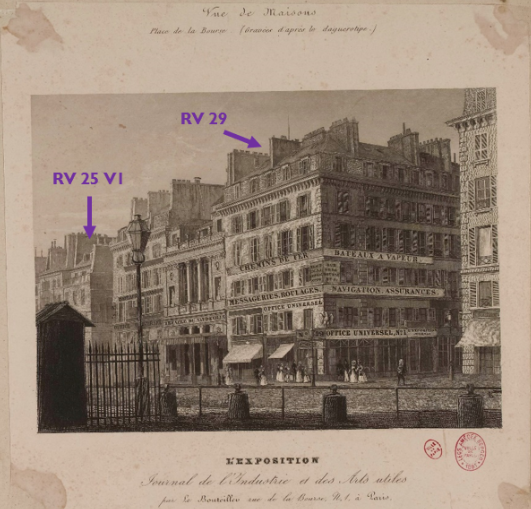
\includegraphics[width=\textwidth]{includes/c_slide7_0.png}
		\end{subfigure}
		\begin{subfigure}{0.48\textwidth}
			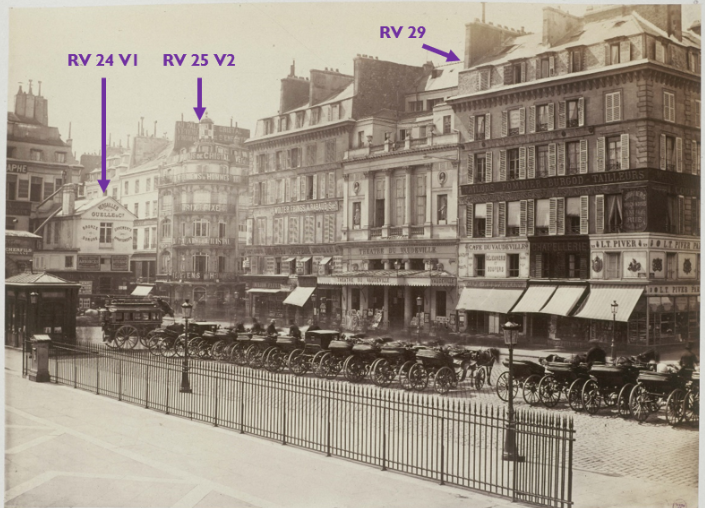
\includegraphics[width=\textwidth]{includes/c_slide7_1.png}
		\end{subfigure}
		\begin{subfigure}{0.48\textwidth}
			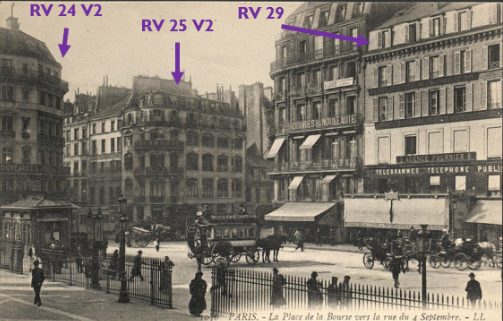
\includegraphics[width=\textwidth]{includes/c_slide7_2.png}
		\end{subfigure}
		\begin{subfigure}{0.48\textwidth}
			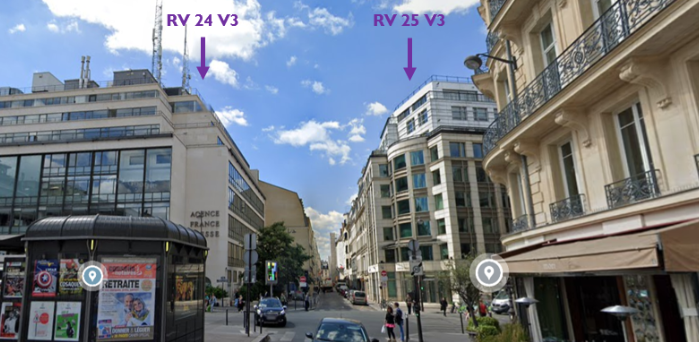
\includegraphics[width=\textwidth]{includes/c_slide7_3.png}
		\end{subfigure}
	\end{figure}
\end{frame}

\subsection{Vers une restitution 3D de la place de la Bourse}
\begin{frame}{Restituer un lieu: des sources à la modélisation 3D}{Vers une restitution 3D de la place de la Bourse}
	\begin{columns}[c]
		\begin{column}{0.45\textwidth}
			Travailler avec des sources photographiques historiques pour la restitution 3D impose de nombreuses contraintes:
			\begin{itemize}
				\item Les tirages peuvent avoir été endommagés et peuvent comporter des défauts liés à leur production ou numérisation
				\item La densité de documents relatifs à un même bâtiment est généralement faible, et celui-ci peut avoir été modifié entre deux clichés
				\item On ne dispose pas de données de calibration internes ou externes associés aux documents, et on doit généralement les déterminer à partir d’une seule image.
			\end{itemize}
		\end{column}
		\begin{column}{0.55\textwidth}
			\begin{figure}
				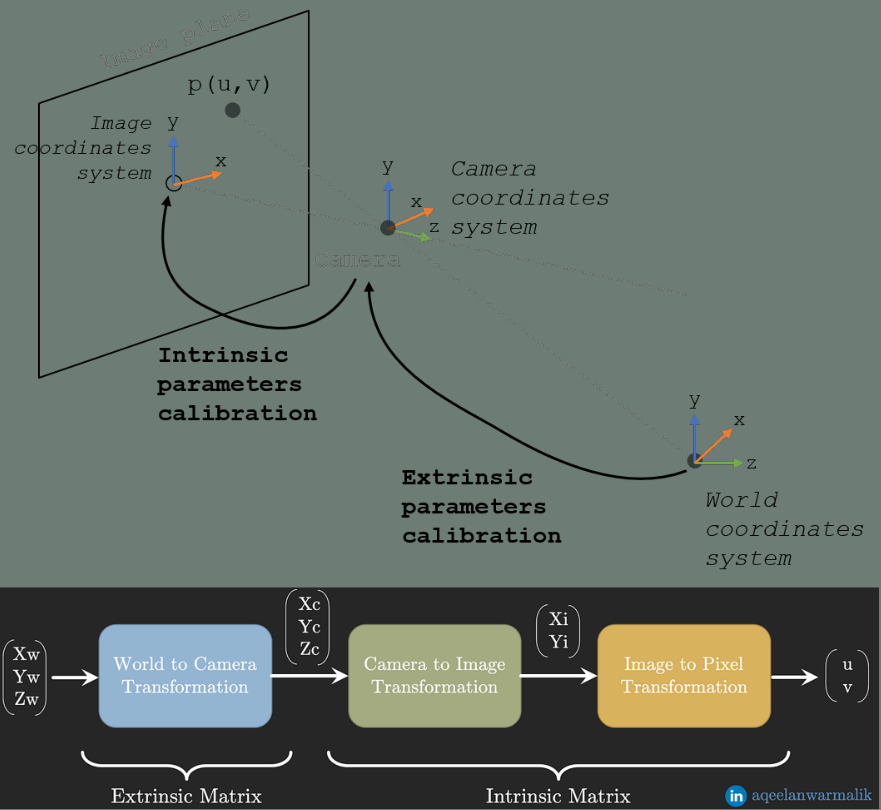
\includegraphics[width=\textwidth]{includes/c_slide8.png}
			\end{figure}
		\end{column}
	\end{columns}
\end{frame}

\begin{frame}{Restituer un lieu: des sources à la modélisation 3D}{Méthodologie}
	\begin{figure}
		\begin{subfigure}{0.25\textwidth}
			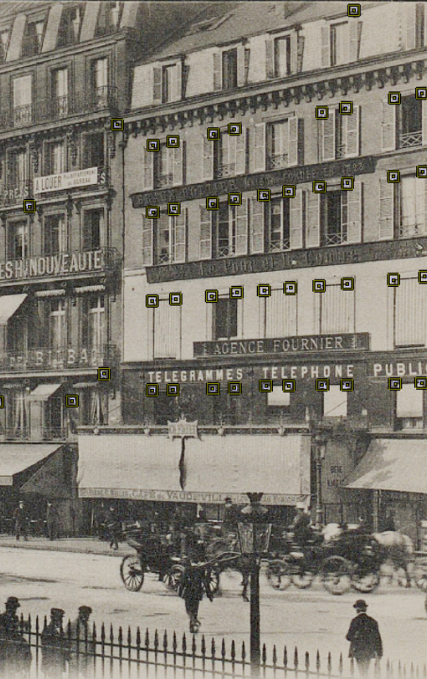
\includegraphics[width=\textwidth]{includes/c_slide9_0.png}
			\caption{Points de contrôle image}
		\end{subfigure}
		\begin{subfigure}{0.23\textwidth}
			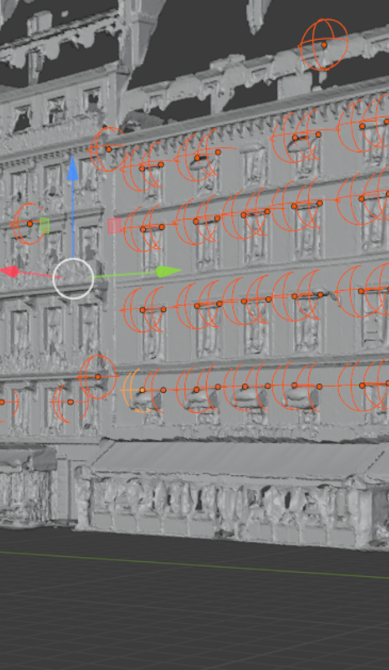
\includegraphics[width=\textwidth]{includes/c_slide9_1.png}
			\caption{Points de contrôle modèle}
		\end{subfigure}
		\begin{subfigure}{0.25\textwidth}
			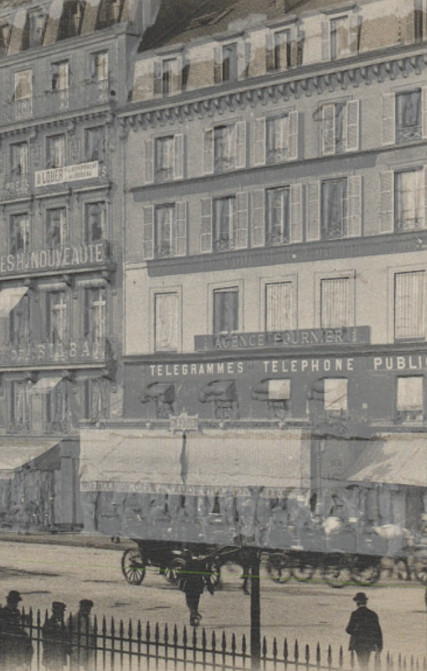
\includegraphics[width=\textwidth]{includes/c_slide9_2.png}
			\caption{Calibration interne et externe}
		\end{subfigure}
		\begin{subfigure}{0.23\textwidth}
			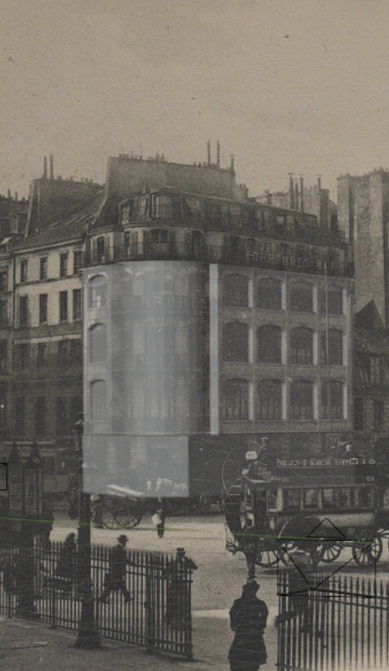
\includegraphics[width=\textwidth]{includes/c_slide9_3.png}
			\caption{Modélisation d'après photographie}
		\end{subfigure}
	\end{figure}
\end{frame}


\begin{frame}{Restituer un lieu: des sources à la modélisation 3D}{Méthodologie}{Limites de perspective}
	\begin{columns}[c]
		\begin{column}{0.5\textwidth}
			La méthode ici présentée présente toutefois un certain nombre d’inconvénients:
			\begin{itemize}
				\item La détermination des paramètres de calibration se fait de manière approchée et n’est pas toujours robuste
				\item L’inclusion d’un plus grand nombre de paramètres à déterminer implique une solution localement précise mais globalement biaisée
				\item Il est souvent nécessaire d’exploiter des photos avec une parallaxe importante pour la restitution, mais celles-ci ne sont pas souvent disponibles
				\item La restitution reste un processus relativement manuel à cause de la difficulté à trouver des points coïncidents entre les photographiess
			\end{itemize}
		\end{column}
		\begin{column}{0.5\textwidth}
			\begin{figure}
				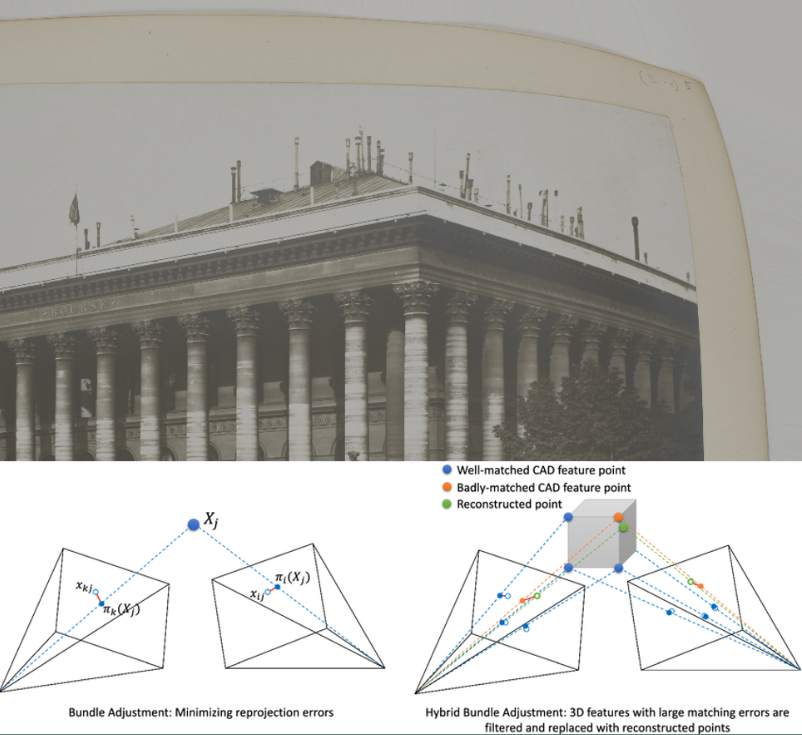
\includegraphics[width=\textwidth]{includes/c_slide10.png}
			\end{figure}
		\end{column}
	\end{columns}
\end{frame}

\section*{Conclusion}
\begin{frame}{Conclusion}
	\begin{figure}
		\begin{subfigure}{0.5\textwidth}
			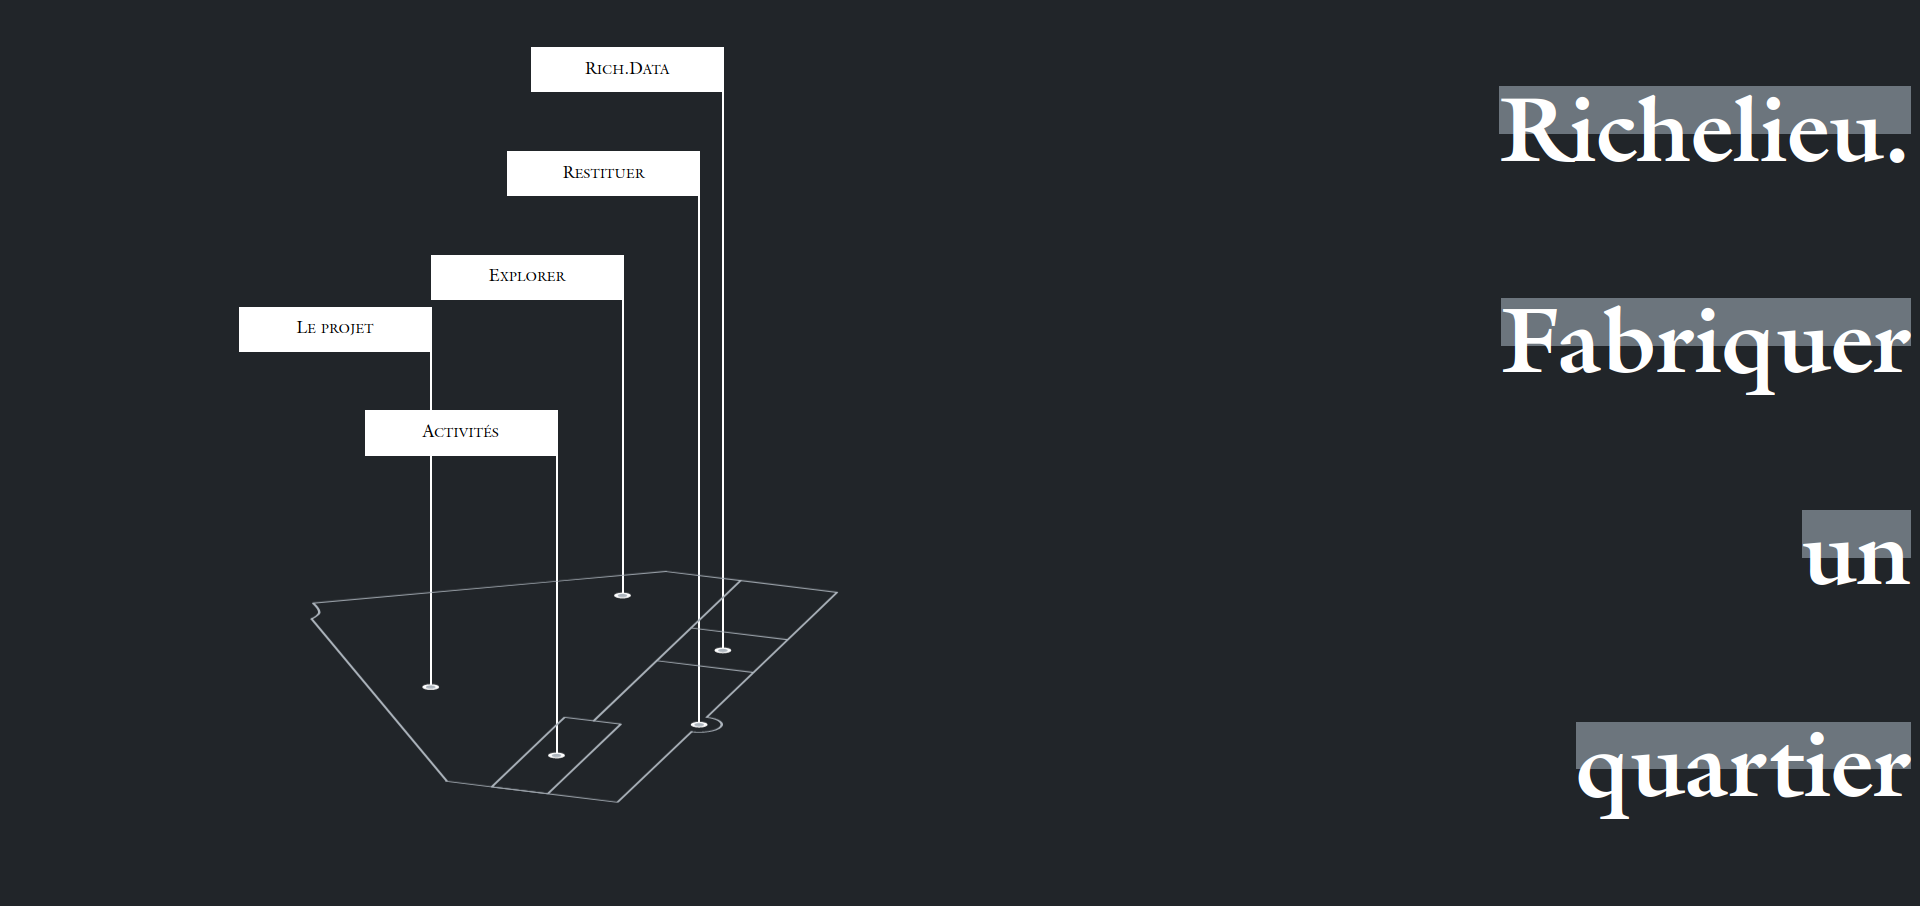
\includegraphics[width=\textwidth]{includes/conclu0.png}
		\end{subfigure}
		\begin{subfigure}{0.5\textwidth}
			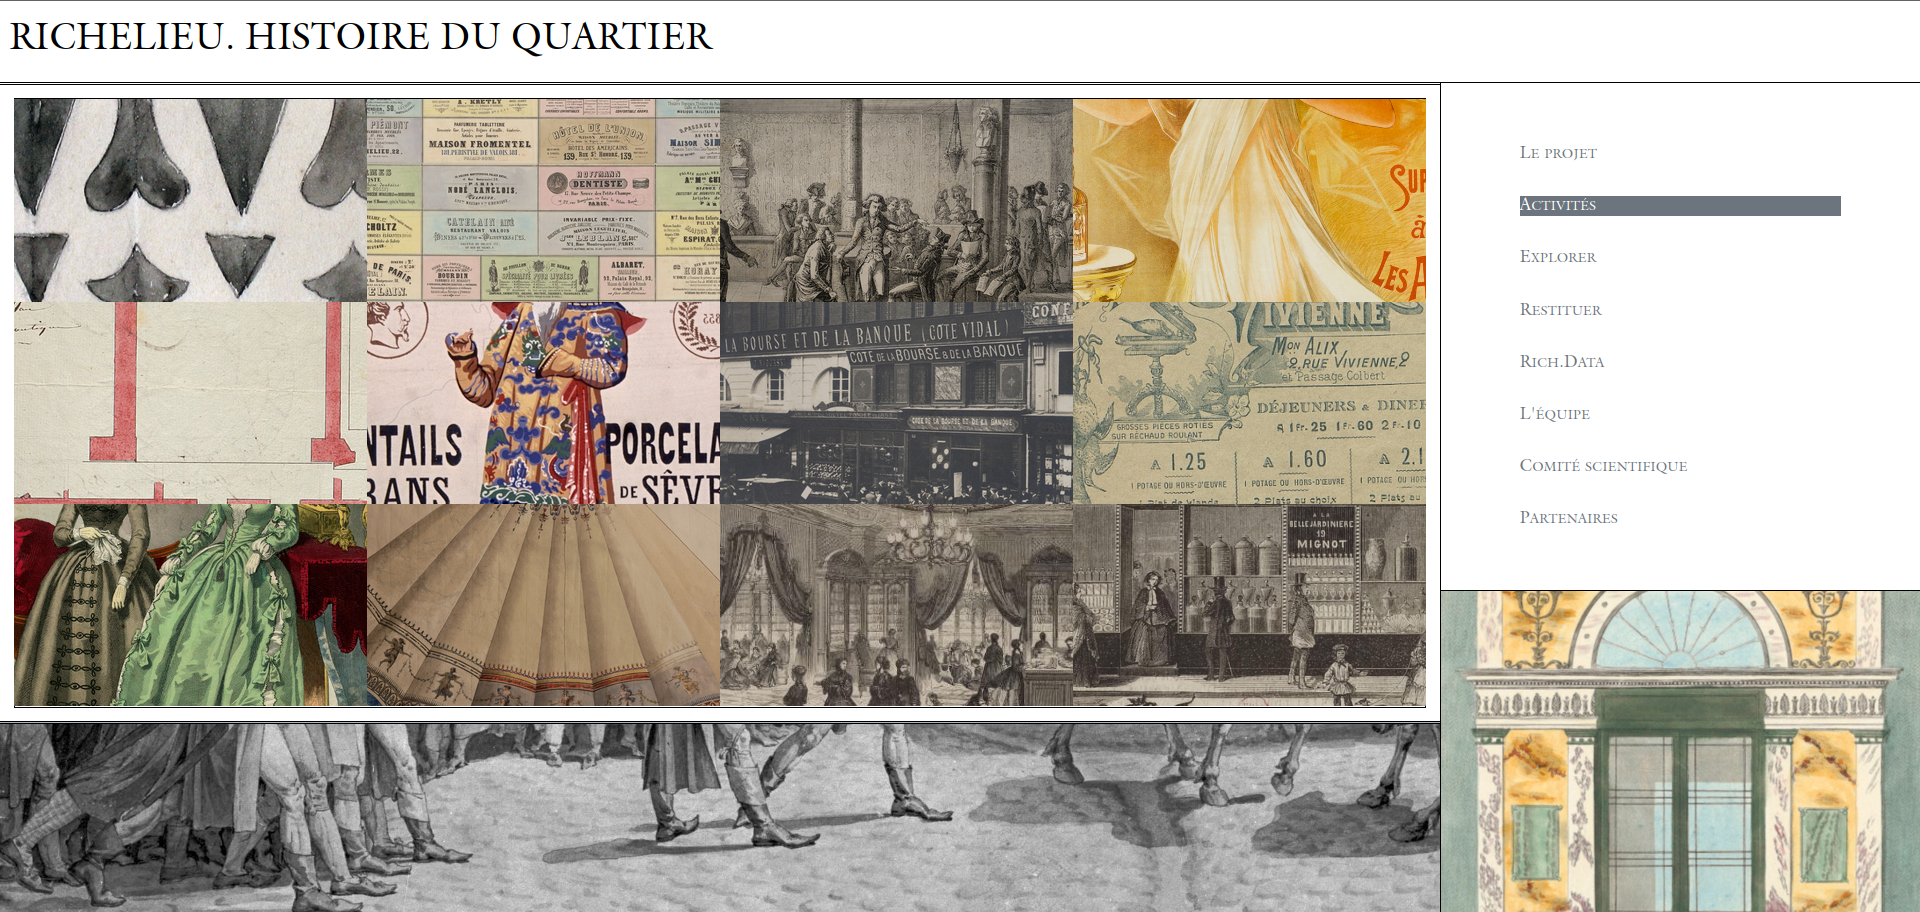
\includegraphics[width=\textwidth]{includes/conclu1.png}
		\end{subfigure}
		\begin{subfigure}{0.5\textwidth}
			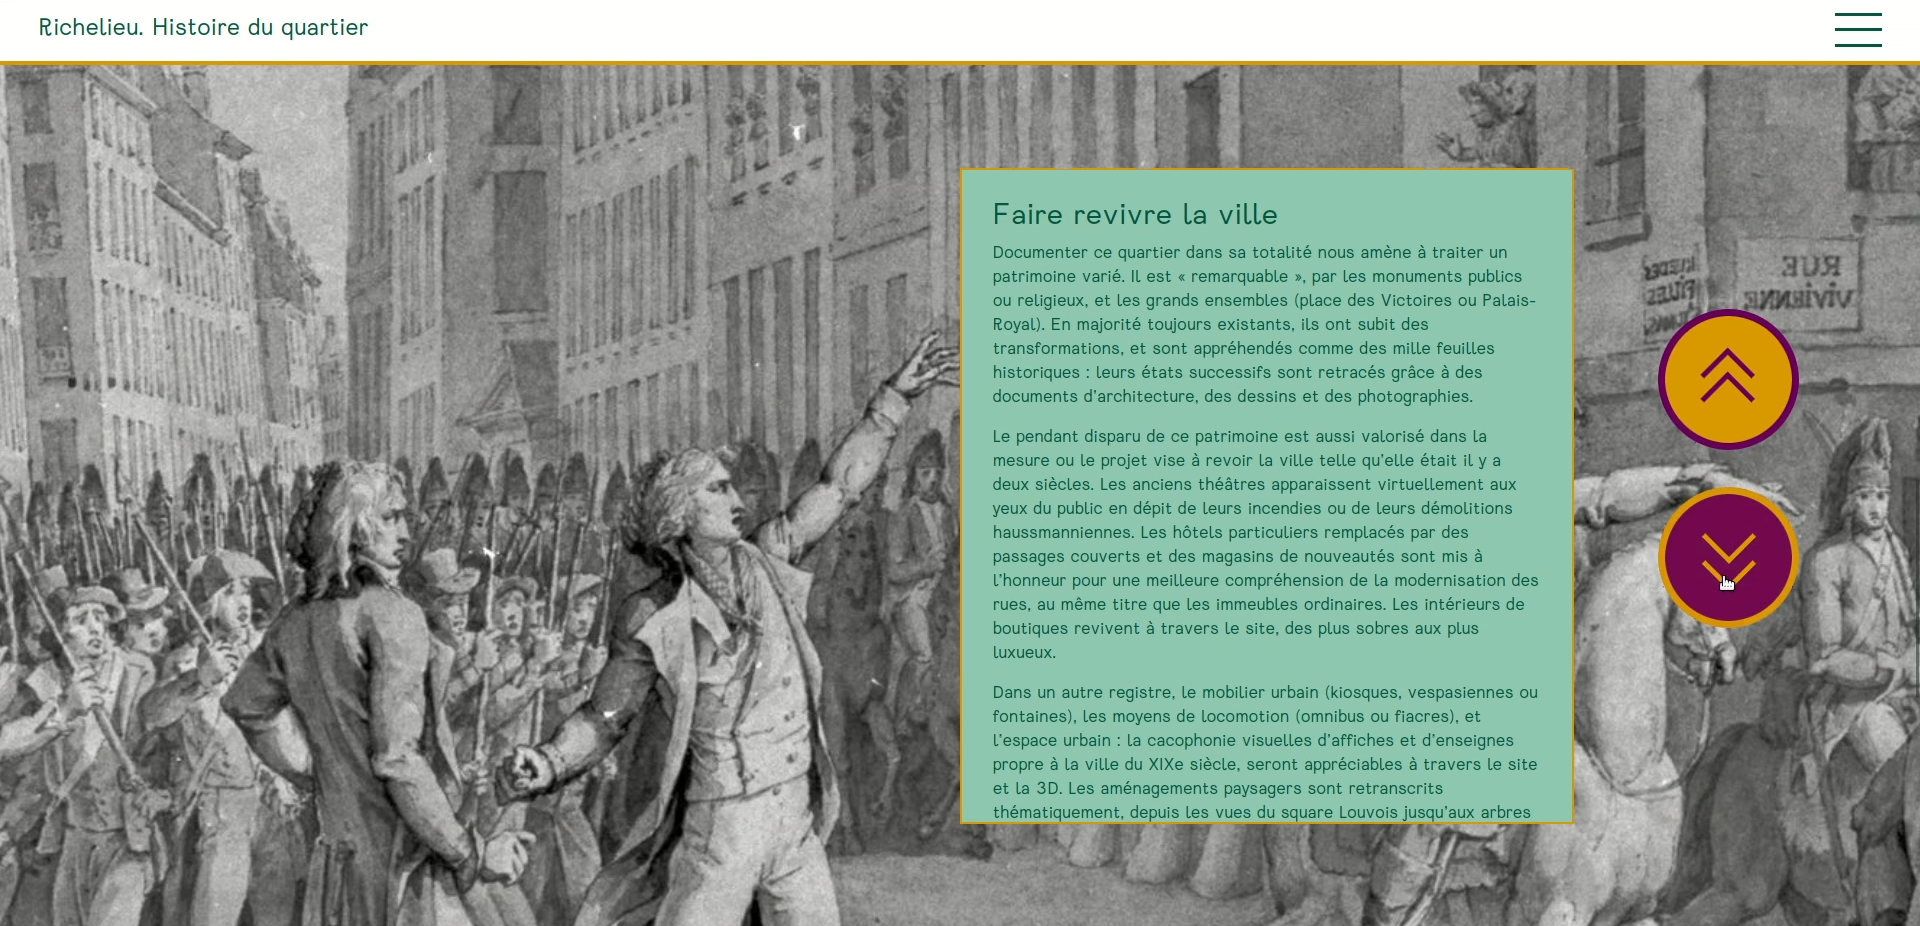
\includegraphics[width=\textwidth]{includes/app_2.png}
		\end{subfigure}
		\caption{Site et application Web du projet Richelieu}
	\end{figure}
	\begin{center}
		Site de présentation du projet:
		\url{https://quartier-richelieu.inha.fr}
	\end{center}
\end{frame}

\end{document}